\documentclass[qo.tex]{subfiles}

\begin{document}
\part{Quantum Theory In Condensed Matter}
\chapter{Bose-Einstein Statistics}
\section{Statistical Ensembles}
In statistical mechanics, one frequently formally considers $N$ copies of the system under consideration. 
Such an assembly is a \emph{statistical ensemble.}
\begin{itemize}
    \item In the \emph{microcanonical ensemble}, each copy has the same total poarticle number $N$ and total energy $U$.
    \item In the \emph{canonical ensemble}, each copy has the same total particle number $N$, however the total energy may fluctuate. 
        The system is considered to be in equilibrium with an external heat bath (maintaining a constant temperature $T$.
    \item In the \emph{grand canonical ensemble}, the total particle number and the total energy may fluctuate. 
        The system is considered to be in equilibrium with an external heat bath, and a particle bath (maintaining a constant chemical potential $\mu$).
\end{itemize}
We are generally interested in macroscopic systems of an effectively infinite number of particles, and may take the \emph{thermodynamic limit} $V\to\infty$ in which the particle density $n=N/V$ is held constant. 
The thermodynamic predictions of the three ensembles are then identical, and it is usually more convenient to use the grand canonical ensemble. 
If the $N$-body quantum states of $N$ quantum particles have energy $E_n^{(N)}$ for $n=1,2,\dots$, then in the grand canonical ensemble, each state occurs with probability
\begin{align}
    P_n^{(N)} &= \frac{1}{Z}\exp\left(-\frac{1}{k_BT}\left[E_n^{(N)}-\mu N\right]\right),
    \text{ where } Z = \sum_{N,k} \exp\left(-\frac{1}{k_BT}\left[E_n^{(N)}-\mu N\right]\right)
\end{align}
is the \emph{grand partition function.}

\section{Particle with Periodic Boundary Conditions}
Consider a point particle of mass $m$ moving within a volume $V=L_xL_yL_z$, where $L_i$ are lengths in the $i=x,y,z$ directions. 
The Hamiltonian 
\begin{equation}
    \hat{H} = \frac{1}{2m}\left(\hat{p}_x^2+\hat{p}_y^2+\hat{p}_z^2\right),
\end{equation}
and the eigenstates of the momentum operator $\hat{p}=(\hat{p}_x,\hat{p}_y,\hat{p}_z)$ are also eigenstates of $\hat{H}$ (subject to periodic boundary conditions).
In the \emph{position representation}, they take the form of plane waves:
\begin{align}
    \psi_k(\vr) = \frac{1}{\sqrt{V}}e^{i\unl{k}\cdot\vr}, \text{ where } \unl{k} = \left(\frac{2\pi n_x}{L_x},\frac{2\pi n_y}{L_y},\frac{2\pi n_z}{L_z}\right).
\end{align}
The differences in $k$ between neighbouring eigenstates are $2\pi/L_i$, in the $i=x,y,z$ directions.
The $k$-space density of the available states is therefore
\begin{align}
    \rho(\unl{k}) = \frac{L_xL_yL_z}{(2\pi)^3} = \frac{V}{(2\pi)^3}.
\end{align}

\section{Spherical Shells in k}
We divide up $k$-space into thin concentric shells. 
A shell of radius $k_S$ and thickness $\delta k_S$ has volume $4\pi k_S^2\delta k_S$, and therefore contains $M_S$ states, where
\begin{align}
    M_S &= 4\pi k_S^2\delta k_S\rho(\unl{k}) = 4\pi k_S^2\delta k_S \frac{V}{(2\pi)^3}.
\end{align}
Each such quantum state has energy $\e_S=\hbar^2k_S^2/2m$, from which we can determine an energy increment $\delta\e_S=(\hbar^2/m)k_S\delta k_S$.
Hence, the number of available states between energies $\e_S$ and $\e_S+\delta\e_S$ is
\begin{align}
    M_S = Vg(\e_S)\delta\e_S, \text{ where } g(\e) = \frac{m^{3/2}}{\sqrt{2}\pi^2\hbar^3}\e^{1/2}
\end{align}
is the (energy) density of states per unit volume. 
\emph{All states on a given shell have the same energy.}

\section{Thermal Equilibrium and the Bose-Einstein Distribution}
Consider an \emph{ideal Bose gas}, i.e. a system of many identical, non-interacting bosons, e.g. in a box subject to periodic boundary conditions. 
In \emph{thermal equilibrium}, the particles are distributed so that the occupation numbers $N_S$ in each shell of energy $\e_S$ maximise the total entropy. 
This yields the \emph{Bose-Einstein distribution:}
\begin{align}
    f_{BE}(\e) = \frac{1}{e^{(\e-\mu)/k_BT}-1}.
\end{align}

\section{Particle Density in the Thermodynamic Limit}
Using the Bose-Einstein distribution in Eq (1.7), the total number of particles in a volume $V$ (subject to periodic boundary conditions) is
\begin{align}
    N &= \sum_{\unl{k}}\frac{1}{e^{(\e_{\unl{k}}-\mu)/k_BT}-1}.
\end{align}
Taking the thermodynamic limit $V\to\infty$, the possible $\unl{k}$ values tend to a continuum, and we replace the sum $\sum_{\unl{k}}$ with an integral $\int\rho(\unl{k})\,dk_x\,dk_y\,dk_z \equiv \int\rho(\unl{k})\,d^3k = [V/(2\pi)^3]\int\,d^3k$.
Hence
\begin{align}
    N &= \frac{V}{(2\pi)^3}\int \frac{d^3k}{e^{(\e_{\unl{k}}-\mu)/k_BT}-1} \implies n \equiv \frac{N}{V} = \frac{1}{(2\pi)^3}\int \frac{d^3k}{e^{(\e_{\unl{k}}-\mu)k_BT}-1}.
\end{align}
Recalling $V/(2\pi)^3\,d^3k = [V/(2\pi)^3]4\pi k^2\,dk = Vg(\e)\,d\e$, then in terms of the density of states per unit volume, $g(\e)$,
\begin{align}
    n = \int \frac{g(\e)\,d\e}{e^{(\e_{\unl{k}}-\mu)/k_BT}-1}.
\end{align}

\chapter{Bose-Einstein Condensation}
\section{Particle Density in Terms of the Fugacity}
Using the fugacity $z\equiv e^{\mu/k_BT}$ and $x\equiv \e/k_BT$, we can rewrite the particle density $n$ as
\begin{align}
    n &= \frac{(mk_BT)^{3/2}}{\sqrt{2}\pi^2\hbar^3}\ofnt \frac{ze^{-x}}{1-ze^{-x}}x^{1/2}\,dx.
\end{align}
Taylor expanding $(1-ze^{-x})^{-1}$ around $ze^{-x}=0$, we deduce the identity
\begin{align}
    ze^{-x}(1-ze^{-x})^{-1} &= ze^{-x}\left(1+ze^{-x}+z^2e^{-2x} + \dots\right) = \sum_{j=1}^\infty z^je^{-jx}.
\end{align}
As $x>0$, this expansion is convergent for $z<1$, and we can evaluate the integral over $x$ using:
\begin{align}
    \ofnt e^{-jx}x^{1/2}\,dx &= \frac{1}{j^{3/2}}\underbrace{\ofnt e^{-y}y^{1/2}\,dy}_{\equiv \Gamma(3/2)} = \frac{1}{j^{3/2}}\frac{\sqrt{\pi}}{2}.
\end{align}
This implies 
\begin{align}
    n &= \left(\frac{mk_BT}{2\pi\hbar^2}\right)^{3/2}g_{3/2}(z), \text{ where } g_{3/2}(z) = \sum_{j=1}^\infty \frac{z^j}{j^{3/2}}.
\end{align}
We therefore need to know something of the properties of $g_{3/2}(z)$ to evaluate the particle density $n$.

\section{Properties of g}
The series defining $g_{3/2}(z)$ converges when $|z|<1$, and diverges when $|z|>1$.
At $z=1$, it is just convergent:
\begin{align}
    g_{3/2}(1) &= \zeta(3/2) = 2.612, \text{ where } \zeta(s) \equiv \sum_{j=1}^\infty \frac{1}{j^s}
\end{align}
is the Riemann zeta function.
The derivative of $g_{3/2}(z)$, however, is infinite at $z=1$, since
\begin{align}
    \frac{d}{dz}g_{3/2}(z)\bigg|_{z=1} &= \frac{1}{z}\sum_{j=1}^\infty \frac{z^j}{j^{1/2}}\bigg|_{z=1} = \sum_{j=1}^\infty \frac{1}{j_{1/2}}
\end{align}
diverges.
With these limiting values, we can make a sketch of $g_{3/2}(z)$ for $0\leq z\leq1$:
\begin{figure}[H]
    \centering
    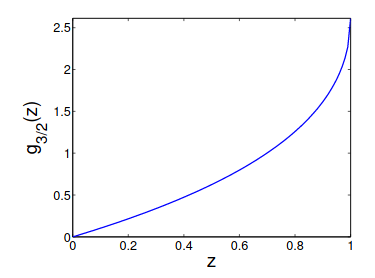
\includegraphics[scale=0.7]{g32.png}
\end{figure}

\section{Critical Temperature}
We can invert Eq (2.4) to get 
\begin{align}
    g_{3/2}(z) &= \left(\frac{2\pi\hbar^2}{mk_BT}\right)^{3/2}n.
\end{align}
If we are in a regime of high $T$ or low $n$, it follows that $g_{3/2}(z)$ must take a small value.
From the plot of $g_{3/2}(z)$ above, we see that this implies small $z$, which from the definition of $g_{3/2}(z)$ means we can approximate $g_{3/2}(z)\approx z$. 
Hence, recalling $z=e^{\mu/k_BT}$,
\begin{align}
    \mu &\approx -\frac32 k_BT\ln\left(\frac{mk_BT}{2\pi\hbar^2n^{2/3}}\right),
\end{align}
i.e., the chemical potential is negative. \\
As $n$ is fixed, it follows from Eq (2.4) that as $T$ is lowered (but assumed $T>0$), $z$ must increase, with maximum finite value of $z=1$, i.e. $\mu=0$.
It straightforwardly follows that this occurs at a \emph{critical temperature} (recalling $g_{3/2}(1)=2.612$) of 
\begin{align}
    T_C &= \frac{2\pi\hbar^2}{k_Bm}\left(\frac{n}{2.612}\right)^{2/3}.
\end{align}

\section{Macroscopic Occupation of the Ground State}
Recall that the Bose-Einstein distribution from Eq (1.7) predicts the occupation of $\e=\e_{\unl{k}=0}=0$ state to be 
\begin{align}
    N_0 &= \frac{1}{e^{-\mu/k_BT}-1}.
\end{align}
Hence, $\mu=0\implies N_0\to\infty$ (Bose-Einstein condensation).
Recalling that we are in the thermodynamic limit ($N,V\to\infty$), what this actually means is that $n_0=N_0/V$ is some finite fraction of $n$.
Rewriting Eq (2.10) for large $N_0$, we obtain 
\begin{align}
    \mu &= -k_BT\ln\left(1+\frac{1}{N_0}\right) \approx -\frac{k_BT}{N_0}.
\end{align}
Hence, as $N_0\to\infty$, $\mu\to0$.
Therefore, below $T_C$, the chemical potential $\mu$ is effectively 0.

\section{Below the Critical Temperature}
Below $T_C$, we must take $\vk=0$ point into account separately, and so we set $\mu=0$ and modify Eq (1.8) to
\begin{align}
    N &= N_0 + \sum_{\vk\neq0}^\infty \frac{1}{e^{\e_{\vk}/k_BT}-1}.
\end{align}
Again, replacing the sum by an integral (excluding $\vk=0$), the particle density is given by 
\begin{align}
    n = n_0 + \frac{(mk_BT)^{3/2}}{\sqrt{2}\pi^2\hbar^3}\ofnt \frac{e^{-x}}{1-e^{-x}}x^{1/2}\,dx.
\end{align}
The integral is identical to that evaluated in Sec (2.1), and so for $T<T_C$, 
\begin{align}
    n &= n_0 + 2.612\left(\frac{mk_BT}{2\pi\hbar^2}\right)^{3/2}.
\end{align}
One speaks of a \emph{condensate density} $n_0$, and a \emph{normal density} $n_n$.
Using the definition of $T_C$ in Eq (2.9), the \emph{condensate fraction} can be compactly written as
\begin{align}
    \frac{n_0}{n} &= 1-\left(\frac{T}{T_C}\right)^{3/2}.
\end{align}
Hence, at $T=0$, all particles are in the ground state, but the proportion decreases to zero as $T\to T_C$ from below, and is zero above $T_C$.

\section{Discontinuity in Heat Capacity Implies Phase Transition}
The heat capacity can be obtained by differentiating the internal energy per particle $u$ while keeping the density $n$ constant:
\begin{align}
    C_V &= \frac{\p u}{\p T}.
\end{align}
The total internal energy $U$ can be determined by multiplying the density of states $g(\e)$ by the volume $V$ and the Bose-Einstein distribution $f_{BE}(\e)$, and then integrating the resulting total energy distribution, multiplied over $\e$, over all values of $\e$:
\begin{align}
    U &= V\ofnt \frac{\e g(\e)\,d\e}{e^{(\e-\mu)/k_BT}-1} = \frac{V(k_BT)^{5/2}m^{3/2}}{\sqrt{2}\pi^2\hbar^3}\ofnt \frac{ze^{-x}}{1-ze^{-x}}x^{3/2}\,dx.
\end{align}
To calculate the average energy per particle, 
\begin{align}
    u &= \frac{U}{N} \equiv \frac{U/V}{N/V},
\end{align}
we use the expression for $n$ in Eq (2.4) to determine (by similar methods as in Sec 2.1), for $T>T_C$,
\begin{align}
    \frac{U}{V} &= \frac{(k_BT)^{5/2}m^{3/2}}{\sqrt{2}\pi^2\hbar^3}\underbrace{\sum_{j=1}^\infty\frac{z^j}{j^{5/2}}}_{\equiv g_{5/2}(z)}\underbrace{\ofnt e^{-y}y^{3/2}\,dy}_{\equiv \Gamma(5/2)},\\
    u &= k_BT\frac{\Gamma(5/2)g_{5/2}(z)}{\Gamma(3/2)g_{3/2}(z)} = \frac{3k_BT}{2}\frac{g_{5/2}(z)}{g_{3/2}(z)},
\end{align}
where we have used the identity $\Gamma(t)=(t-1)\Gamma(t-1)$.
Note that $g_{5/2}(z)$ and $g_{3/2}(z) \to z$ as $z\to0$, and so $\mu\approx \frac32 k_BT$ when $T\gg T_C$, i.e. the classical result. \\
For $T<T_C$, we use $n$ as given by Eq (2.9), and determine
\begin{align}
    u &= \frac{3k_B}{2}\frac{T^{5/2}}{T^{3/2}_C}\frac{g_{5/2}(1)}{g_{3/2}(1)},
\end{align}
where $g_{5/2}(1)=\zeta(5/2)=1.342$.\\
For $T\gg T_C$, we obtain the classical result
\begin{align}
    C_V &= \frac{\p u}{\p T} \approx \frac32 k_B;
\end{align}
while for $T<T_C$,
\begin{align}
    C_V &+ \frac{15}{4}\frac{g_{5/2}(1)}{g_{3/2}(1)}\left(\frac{T}{T_C}\right)^{3/2}k_B.
\end{align}
When plotted as a function of $T$, the curves for $T<T_C$ and $T>T_C$ meet at a cusp (discontinuity in slope).
This implies that the free energy is not analytic at $T_C$, and so BEC is a true thermodynamic \emph{phase transition.}

\emph{doodle plot from visualiser}


\chapter{BEC in Ultracold Dilute Gases of Alkali Atoms}
\section{Bosonic Alkali Atomic Gases}
Alkali metals are group 1 elements, and have a single valence electron in the outermost $s$-orbital: $2s$ for Li, $3s$ for Na, $4s$ for K, $5s$ for Rb. 
The other electrons are in fully occupied shells, and therefore have total orbital and spin angular momentum $=0$.
If the isotope is such that the nucleus is composed of an odd total number of protons and neutrons, the nucleus will have a net half-integer spin ($=\frac32$ for $^{87}$Rb, $^{23}$Na, $^7$Li).
The \emph{total spin} will then take an integer value ($=1,2$ for $^{87}$Rb, $^{23}$Na, $^7$Li).
It is possible to prepare the gas such that only one of these states is present, which can be considered a gas of identical particles having integer spin, i.e. \emph{identical bosons.}

\section{Critical Temperature}
Densities of trapped atomic gases are typically $\approx10^{11}-10^{15}$cm$^{-3}$. 
Using such values and appropriate atomic masses to determine $T_C$ for the \emph{ideal, homogeneous} Bose gase yield $T_C$ between 10 nanoKelvin and 1 microKelvin.
Such temperatures can be achieved relatively straightforwardly by methods of laser and evaporative cooling; BEC was first observed in 1995 in magnetically trapped gases of $^{87}$Rb and $^{23}$Na (Nobel prize in physics 2001).

\section{Atom-Atom Interactions}
The atoms interact with each other, and so we do not have an ideal Bose gas (interactions are in fact essential to establish thermal equilibrium during cooling).
Interactions are dominated by elastic two-body collisions (in such dilute gases, the probability of 3 atoms meeting at the same point in space is extremely low).
No binding takes place in elastic collisions, and so atomic clusters do not tend to form. 
At the very cold temperatures under consideration, the collisions are very low energy, and the pair-interaction may be approximated by
\begin{align}
    V(\vr-\vr') &\approx g\delta(\vr-\vr'), \text{ where } g = \frac{4\pi\alpha_s\hbar^2}{m},
\end{align}
and $\alpha_s$ is the $s$-wave scattering length. 

\section{Mean-Field Potential}
Usually $\alpha_s$ is positive, implying a net repulsive interaction. 
On average this can be represented by an additional potential, proportional to the \emph{atomic density} $n(\vr)$, felt by each particle due to its interaction with all other particles:
\begin{align}
    V_{\text{eff}}(\vr) &= gn(\vr).
\end{align}
In this approximation, the trapped atoms obey an effective Schrodinger equation,
\begin{align}
    H_{\text{eff}}\psi(\vr) &= \left[-\frac{\hbar^2}{2m}\del^2 + V_{\text{trap}}(\vr) + V_{\text{eff}}(\vr)\right] \psi(\vr) = \e\psi(\vr),
\end{align}
where the trapping potential $V_{\text{trap}}(\vr)$ can usually be considered harmonic. 
Finding the steady states $\psi(\vr)$ and their corresponding "eigenvalues" $\e$ is not simply a matter of diagonalising $H_{\text{eff}}$ however, as $V_{\text{eff}}(\vr)$ is dependent on the state of the system, i.e. the effective Schrodinger equation is \emph{non-linear.}

\section{Gross-Pitaevskii Equation}
An appropriate thermodynamic limit is to let $N\to\infty$ while relaxing the trap.
If 
\begin{align}
    V_{\text{trap}}(\vr) &= \frac{m\om^2 r^2}{2},
\end{align}
mathematically this corresponds to keeping $N\alpha_s/\alpha_h$ constant, as while letting $N\to\infty$,
\begin{align}
    \alpha_h &\equiv \sqrt{\frac{\hbar}{m\om}}\to\infty.
\end{align}
Below a critical temperature $T_C$, a transition to a "macroscopically occupied" quantum state occurs, but the mode (i.e. the spatical dependency of this state) changes with varying $T<T_C$ due to the combination of $V_{\text{trap}}(\vr)$ and atom-atom interactions.
In the thermodynamic limit and as $T\to0$, all but a vanishingly small proportion of atoms enter a "ground state" mode $\psi_0(\vr)$, which obeys the \emph{Gross-Pitaevski equation}:
\begin{align}
    \left[-\frac{\hbar^2}{2m}+V_{\text{trap}}(\vr)+gN|\psi_0(\vr)|^2\right]\psi_0(\vr) = \e_0\psi_0(\vr).
\end{align}
This is a very useful equation for typical atom numbers $(\approx 10^3-10^8)$.

\section{Thomas-Fermi Limit}
Consider $V_{\text{trap}}(\vr) = m\om^2r^2/2$.
All other things being equal, of $gN$ is allowed to become very large (this corresponds to letting $N\alpha_s/\alpha_h\to\infty$), the kinetic energy is completely dominated over most of the mode bby the potential energy. 
Hence,
\begin{align}
    \left[\frac{m\om^2r^2}{2}+gN|\psi_0(\vr)|^2\right]\approx \e_0.
\end{align}
We can therefore determine a limiting spatial dependency of $\psi_0(\vr)$:
\begin{align}
    \psi_0(\vr) &= \begin{cases} \sqrt{\frac{\e_0-m\om^2r^2/2}{gN}} & \text{if } r\leq\sqrt{\frac{2\e_0}{m\om^2}}, \\ 0 & \text{if } r > \sqrt{\frac{2\e_0}{m\om^2}}, \end{cases}
\end{align}
and knowing the norm of $\psi_0(\vr)$ must be 1, one can show that in this limit
\begin{align}
    \e_0 &= \left(\frac{15gN}{8\pi}\right)^{2/5}\left(\frac{m\om^2}{2}\right)^{3/5}.
\end{align}

\section{Hydrodynamic Formulation}
To a good approximation, the atomic condensate dynamics can frequently be described by the \emph{time dependent} Gross-Pitaevskii equation:
\begin{align}
    i\hbar\dpt\psi(\vr) &= \left[-\frac{\hbar^2}{2m}\del^2 + V_{\text{trap}}(\vr) + gN|\psi(\vr)|^2\right]\psi(\vr).
\end{align}
Defining the probability density $\rho(\vr)=|\psi(\vr)|^2$ and a velocity field
\begin{align}
    \vec{v}(\vr) &= \frac{\hbar}{2im\rho(\vr)}\left[\psi^*(\vr)\del\psi(\vr) - \psi(\vr)\del\psi^*(\vr)\right],
\end{align}
it is possible to formulate a hydrodynamic description. 
The (coupled) equations of motion are the \emph{continuity equation},
\begin{align}
    \dpt\rho(\vr) &= -\del\cdot\left[\rho(\vr)\vec{v}(\vr)\right],
\end{align}
and the equation of motion for the velocity field,
\begin{align}
    m\dpt\vec{v}(\vr) &+ -\del\left[\frac{m}{2}\vec{v}(\vr)^2 + V_{\text{trap}}(\vr) + gN\rho(\vr) - \frac{\hbar^2}{2m\sqrt{\rho(\vr)}}\del^2\sqrt{\rho(\vr)}\right].
\end{align}
If the density is relatively smooth, the final term above can be neglected. 
In this case, together with the continuity equation, we have a dynamical description of a fluid with \emph{zero viscosity}, i.e. \emph{a superfluid}.
When considering a fluid, one would typically not have a $V_{\text{trap}}(\vr)$ term, and it would also be more usual to write the equations in terms of $n(\vr)=N\rho(\vr)$, i.e. the condensate number density, in the present context.

\chapter{Classical and Quantum Fluids}
\section{Characteristic Properties of Classical and Quantum Fluids}
A \emph{fluid} freely deforms or \emph{flows}, i.e. a gas or liquid. 
In normal (classical) fluids, their physical properties are determined from classical statistical mechanics.
A \emph{quantum fluid} remains fluid at sufficiently low temperatures for the effects of quantum mechanics to have a dominant role. 

\section{Statistical Mechanics of Classical Interacting Many-Body Systems}
The classical Hamiltonian for $N$ mass $m$ interacting identical point particles is
\begin{align}
    H(\vec{p}_1,\dots,\vec{p}_N,\vr_1,\dots,\vr_N) &= \frac{1}{2m}\sum_{k=1}^N \vec{p}_k^2 + \frac12\sum_{j\neq k=1}^N V(\vr_j-\vr_k).
\end{align}
The probability of each possible configuration is given by the Boltzmann probability density for $N$ particles and temperature $T$,
\begin{align}
    P(\vec{p}_1,\dots,\vec{p}_N,\vr_1,\dots,\vr_N) &= \frac{1}{Z_N}e^{-H/k_BT}, \\ 
    \text{where } Z_N &= \left(\frac{1}{N!}\right)\int e^{-H/k_BT}\,d^3p_1\dots d^3p_N\,d^3r_1\dots d^3r_N
\end{align}
is the \emph{classical partition function}. 
The $\frac{1}{N!}$ accounts for the particles' indistinguishability. 
$Z_N$ factorises into position- and momentum-dependent terms:
\begin{align}
    Z_N &= \left(\prod_{k=1}^N \int e^{-p_k^2/2mk_BT}\,d^3p_k\right)Q_N = \left(2\pi mk_BT\right)^{3N/2}Q_N, \\
    \text{where } Q_N &= \left(\frac{1}{N!}\right)\int \exp\left(-\sum_{j\neq k=1}^N \frac{V(\vr_j-\vr_k)}{2k_BT}\right)\,d^3r_1\dots d^3r_N.
\end{align}
The momentum part of $Z_N$ is a product of independent individual particle terms. 
Hence, individual particle momenta are statistically independent, and a particle has momentum which is in a region $d^3p$ of momentum space with probability
\begin{align}
    P(\vec{p})\,d^3p &= \frac{e^{-p^2/2mk_BT}}{(2\pi mk_BT)^{3/2}}\,dp.
\end{align}
The fraction of particles with momentum \emph{magnitude} between $p$ and $p+dp$ is
\begin{align}
    P_{MB}(p)\,dp &= \frac{4\pi p^2e^{-p^2/2mk_BT}}{(2\pi mk_BT)^{3/2}}\,dp,
\end{align}
where $P_{MB}(p)$ is the \emph{Maxwell-Boltzmann} momentum distribution.

\section{Interactions in Helium and the Noble Gases}
The atoms interact predominantly via a pairwise interaction potential $V(r)$, where $r$ is the \emph{relative coordinate} describing the distance between atoms.
$V(r)$ contains a short-ranged repulsion and a weak, long-range van der Waals attraction, and it can be sufficient to consider a \emph{Lennard-Jones} model potential:
\begin{align}
    V(r) &= \e_0\left[\left(\frac{r_0}{r}\right)^{12}-2\left(\frac{r_0}{r}\right)^6\right],
\end{align}
where $\e_0$ is the potential depth, and $r_0$ is the position of the potential minimum.

\section{Thermal de Broglie Wavelength}
The de Broglie wavelength is defined as 
\begin{align}
    \lambda &= \frac{2\pi\hbar}{p}.
\end{align}
For a finite temperature system, a characteristic length scale is set by the \emph{thermal de Broglie wavelength},
\begin{align}
    \lambda_{dB} &= \frac{2\pi\hbar}{\sqrt{2\pi mk_BT}} = \sqrt{\frac{2\pi\hbar^2}{mk_BT}}.
\end{align}
$\lambda_{dB}$ corresponds to a momentum $\sqrt{2\pi mk_BT}$, which is distinct from both the \emph{mean} momentum \\ $\sqrt{8mk_BT/\pi}$ and the \emph{most probable} momentum $\sqrt{2mk_BT}$.
Quantum effects should be significant once $\lambda_{dB}$ is comparable to other typical length scales in the fluid. 

\section{Significance of Quantum Effects in the Liquid Phase(s)}
At standard atmospheric pressure, Neon (atomic mass 20) liquifies at $\approx27\,$K and freezes at $\approx24\,$K.
The $\lambda_{dB}\approx0.07\,$nm is much less than $r_0=0.296\,$nm, and quantum effects are unimportant throughout the gas and liquid phases. 
Helium 4 (atomic mass 4) liquifies at $4\,$K.
There are two liquid phases (He I and He II) and no solid phase at standard atmospheric pressure. 
Hence $\lambda_{dB}\approx0.4\,$nm is comparable to $r_0=0.264\,$nm, ad quantum effects are significant.

\section{Phenomenological Low Temperature Model of a Solid Phase}
Assume each atom vibrates with angular frequency $\om_0$ around its equilibrium position in a crystal lattice as an independent quantum harmonic oscillator, with zero-point energy per atom,
\begin{align}
    E_0 &= \frac32\hbar\om_0.
\end{align}
Assume a face-centred cubic lattice structure (12 nearest neighbours, equivalent to 4 springs of spring constant $k$ acting in each of the $x,y,$ and $z$ directions).
The spring constant $k$ (and hence $\om_0=\sqrt{4k/m}$) can be taken from the second-order coefficient from a Taylor expansion of a Lennard-Jones potential about the equilibrium position $r_0$:
\begin{align}
    k &= \frac12 \frac{d^2V(r)}{dr^2}\bigg|_{r=r_0} = \frac{36\e_0}{r^2_0}.
\end{align}

\section{Absence of a Solid Phase in Helium}
From this simple model, for Neon ($\e_0=3.94\,$meV, $r_0=0.296\,$nm), the zero-point energy 
\begin{align}
    E_0 &\equiv 3\hbar\sqrt{\frac{36\e_0}{mr_0^2}}\approx 4\,\text{meV},
\end{align}
which is comparable to $\e_0$.
Thus Neon supports a solid phase. 
For Helium ($\e_0=1.03\,$meV, $r_0=0.265\,$nm), this yields a zero-point energy $E_0\approx7\,$meV which is must greater than the potential well depth $\e_0$, and there is no solid phase. 

\section{Singularity in Heat Capcity/Specific Heat as a Function of Temperature}
Plotting $C_V$ as a function of $T$, at the boundary between the He I and He II phases ($T=T_C=2.17\,$K) one observes a singularity, known as the \emph{lambda point} (due to the alleged resemblance of such a plot near $T_C$ to the letter $\lambda$).
At low $T$, $C_V\propto T^3$ (unlike BEC).
Near $T_C$, $C_V$ has a weak power law behaviour:
\begin{align}
    C_V &= \begin{cases} C(T) + A_+|T-T_C|^{-\alpha}, & T > T_C, \\ C(T) + A_-|T-T_C|^{-\alpha}, & T < T_C,\end{cases}
\end{align}
where $C(T)$ is a smooth function of $T$ near $T_C$.
Within the theory of phase transitions, measured values of the \emph{critical exponent} $\alpha(=-0.009)$, $A_+$, and $A_-$ are consistent with this phase transition belonging to a \emph{universality class} known as the three-dimensional XY-model. 
The \emph{order} of such systems is described by a two-dimensional unit vector at every point in space $\vec{n}(\vr)$.
In He I, this vector is spatially random; in He II, there is a spatial ordering, like the ordering in a ferromagnet. 

\section{The Macroscopic Wavefunction}
A two-dimensional unit vector can be equivalently described by the phase of a \emph{complex number}, such as the Gross-Pitaevskii wavefunction, motivating the introduction of a similar macroscopic wavefunction $\psi_0(\vr)$ here. 
The wavefunction corresponds to a \emph{condensate}, or macroscopic number of particles. 
We can normalise $\psi_0(\vr)$ such that 
\begin{align}
    n_0 &= |\psi_0|^2 \text{ is the condensate density,} \\
    N_0 &= n_0V = \int |\psi_0(\vr)|^2\,d^3r \text{ is the number of condensed particles, and} \\
    \psi_0(\vr) &= \sqrt{n_0(\vr)}e^{i\theta(\vr)}.
\end{align}
If $|\psi_0(\vr)|=0$, the phase $\theta(\vr)$ is undefinedl if $|\psi_0(\vr)|\neq0$, the phase $\theta(\vr)$ is a natural parameter of the system. 
$\psi_0(\vr)$ is the \emph{order parameter} of the He II phase. 

\chapter{Superfluiditity in Helium II}
\section{Superfluid Viscosity}
Assuming a macroscopic wavefunction $\psi_0(\vr)=\sqrt{n_0}e^{i\theta}$, we define the \emph{superfluid velocity} $\vec{v}_s$, which defines a \emph{current density} (particle flow) $\vec{j}_0=n_0\vec{v}_s$.

\section{Superflow and Viscosity}
A normal fluid's flow viscosity $v$ through a (length $L$, radius $R$) capillary depends on the fluid's viscosity $\eta$ and the pressure difference $\Delta P = P_1-P_2$, such that
\begin{align}
    \frac{\Delta P}{L} &\approx \eta\frac{v}{R^2}.
\end{align}
\textbf{Piotr Kapitza} found that with He II, $\Delta P$ was always 0 whatever the value of $v$.
\emph{Superflow} is therefore fluid flow with \emph{zero viscosity}.\\
Alternatively, consider a disc suspended in fluid and made to undergo torsional oscillations about its axis. 
The oscillation frequency depends on the torsional stiffness of the support, and the moment of inertia of the disc. 
In a viscous fluid, a thin layer of fluid is dragged along with the disc's motion, effectively increasing the intertia of the disc. 
With a stack of closely spaced discs, all fluid between the discs should be dragged along, contributing to the inertia. 
Immersing a stack of discs in He II, \textbf{Elepter Andronikashvili} showed that a temperature-dependent fraction of He II contributed to the intertia but a fraction did not. 
This motivated a \emph{two fluid} model of He II.

\section{Two Fluid Model}
The total particle density of the fluid is $n=n_s+n_n$, and the \emph{normal component} $n_n$ acts like a conventional viscous fluid. 
It contributes to the inertia of the rotating discs, but friction with the walls prevents flow down the capillary. 
The superfluid component $n_s$ flows with zero viscosity. 
It does not contribute to the inertia of the rotating discs, but flows freely down the capillary.
The two fluid components move relative to each other without friction. 

\section{Temperature Dependence of the Superfluid and Normal Components}
As $T\to0$, almost all fluid is superfluid, i.e. $n_s\approx n,n_n\approx0$, and near $T=0$ the temperature dependence is $n_s(T)\approx n-AT^4$ (A is a constant).
Near the critical temperature $T_C$ nearly all the fluid is normal, and it is observed experimentally that $n_s$ vanishes like a power law:
\begin{align}
    n_s &\approx \begin{cases} B(T_C-T)^a & T<T_C, \\ 0 & T>T_C, \end{cases}
\end{align}
where the critical exponent $a\approx0.67$ (again consistent with predictions based on the three-dimensional XY model) and $B$ is another constant.

\section{Two Fluid Hydrodynamical Quantities}
The \emph{superfluid density} is the mass density of the superfluid component $\rho_s=mn_s$.
There are two types of current flow, so that the total current density $\vec{j}=\vec{j}_s+\vec{j}_n$, where
\begin{align}
    \vec{j}_s &= n_s\vec{v}_s, & \vec{j}_n &= n_n\vec{v}_n,
\end{align}
and $\vec{v}_s,\vec{v}_n$ are the velocities of the two fluid components.

\section{Flow Quantisation}
From the definition of superfluid velocity, we have $\vec{v}_s = \frac{\hbar}{m}\grad\theta$.
Hence, 
\begin{align}
    \grad\times\vec{v}_s &\equiv \frac{\hbar}{m}\grad\times\grad\theta=0,
\end{align}
i.e. the flow is \emph{irrotational}.
Consider a flow around the inside of a torus, in particular a closed path going all the way around the torus exactly once. 
The flow circulation $\kappa$ is defined by the integral
\begin{align}
    \kappa &= \oint \vec{v}_s\cdot\,d\vr = \frac{\hbar}{m}\oint \grad\theta\cdot\,d\vr = \frac{\hbar}{m}\Delta\theta,
\end{align}
where $\Delta\theta$ is the phase change after having traversed the path. 
The value of any such line integral of $\vec{v}_s$ should be \emph{independent} of the (topologically similar) path between two endpoints. 
Hence, $\Delta\theta$ is the same for any path wrapping around the torus exactly once. 
If $\psi_0(\vr)$ is to be single-valued, we must have $\psi_0(\vr)=\psi_0(\vr)e^{i\Delta\theta}$, i.e. $\Delta\theta=2\pi j$ where $j$ is an integer. 
Hence $\kappa=\frac{h}{m}j$ is quantised in units of $\frac{h}{m}$.

\section{Phase Slips and Persistent Currents}
Consider liquid Helium, at rest ($\kappa=0\implies j=0$) and trapped between two concentric cylinders.
Rotating the cylinders accelerates the normal component until it has the same angular velocity as the apparatus, but leaves the superfluid component at rest.
If the system is then cooled slowly, particles from the normal fluid will gradually be added to the superfluid component.
Hence, their angular momentum will be transferred to the superfluid component, which will begin to rotate.
The circulation $\kappa$ is observed to increase in sudden jumps of $\frac{h}{m}$, called \emph{phase slip} events.
These correspond to changes in the quantum number $j$, and are therefore analagous to transitions between quantum states in an atom. 
Conversely, cooling an initially rotating normal fluid below $T_C$ yields a circulating superflow. 
Without viscosity, in principle this flow continues indefinitely. 

\section{Irrotational Flow and Vortices}
Consider a cylindrical container of liquid Helium. 
In this case (topological considerations would appear to be absent), the irrotational flow condition $\grad\times\vec{v}_s=0\implies\oint\vec{v}_s\cdot\,d\vr=0$ around any closed path.
A \emph{vortex}, however, can satisfy $\grad\times\vec{v}_s=0$ almost everywhere and still allow a net rotation. 
In cylindrical polar coordinates,
\begin{align}
    \grad\times\vec{v}_s &= \frac{1}{r}\begin{vmatrix}\ve_r & r\ve_\phi & \ve_z \\ \frac{\p}{\p r} & \frac{\p}{\p\phi} & \frac{\p}{\p z} \\ v_r & rv_\phi & v_z\end{vmatrix}.
\end{align}
A circulating flow with cylindrical symmetry will obey $\grad\times\vec{v}_s=0$ if $\frac{1}{r}\frac{\p rv_\phi}{\p r}=0$.
The flow velocity around the vortex must therefore be of the form
\begin{align}
    \vec{v}_s &= \frac{\kappa}{2\pi r}\ve_\phi,
\end{align}
where $\kappa$ is the (quantised) net circulation. 
In practice only the lowest energy ($j=\pm1$) vortices are observed.

\section{Vortex Core}
Eq (5.7) satisfies $\grad\times\vec{v}_s=0$ except at $r=0$, the \emph{vortex core} (in Helium, the core region is $\approx1$\AA).
In the vortex core $\psi_0(0)=0$, and so $\theta$ is undefined there.
Hence $n_s\equiv|\psi_0(0)|^2=0$ at the core, and also the superfluid current density $\vec{j}_s\equiv n_s\vec{v}_s=0$.
This avoids any singularity in the supercurrent at the centre of the vortex (topological considerations are thus not entirely absent).
Superfluid Helium inside a rotating cylinder manifests a centrifugally curved free surface, implying circulation.
The \emph{net circulation provided by many vortices}, circumventing a naive interpretation of the irrotationality conditions, explains this.

\section{Vortex Density of a Superfluid in a Rotating Cylinder}
If the cylinder has radius $R$ and angular velocity $\om$, the total circulation around the cylinder boundary will be the velocity at the boundary multiplied by the diameter, i.e. taking the integration contour around the cylinder boundary,
\begin{align}
    \kappa &= \oint \vec{v}_s\cdot\,d\vr = (\om R)(2\pi R).
\end{align}
The circulation is quantised; if there are $N_v$ vortices with $j=1$, then it follows that $\kappa=\frac{h}{m}N_v$.
Hence, the number of vortices per unit area is
\begin{align}
    \frac{N_v}{\pi R^2} &= \frac{2m\om}{h}.
\end{align}
At low rotation rates, vortices from ordered triangular arrays.

\chapter{Interactions and Excitations in Helium II}
\section{Interacting Many-Body Quantum Systems}
Considering pairwise interactions only, the quantum-mechanical Hamiltonian for $N$ interacting particles is given in the position representation by 
\begin{align}
    \Ham = -\sum_{j=1}^N \frac{\hbar^2}{2m}\grad_j^2 + \frac12\sum_{j\neq k=1}^N V(\vr_j-\vr_k).
\end{align}
$\Ham$ acts on $N$-particle wavefunctions of the form $\Psi(\vr_1,\vr_2,\dots,\vr_N)$.
If the particles are bosons, the wavefunction must be \emph{symmetric} under particle exchange, i.e.
\begin{align}
    \Psi(\dots,\vr_j,\dots,\vr_k,\dots) &= \Psi(\dots,\vr_k,\dots,\vr_j,\dots).
\end{align}
In general, a basis of $N$-body energy eigenfunctions $\Psi_n^{(N)}(\vr_1,\vr_2,\dots,\vr_N)$ exists, such that 
\begin{align}
    \Ham\Psi(\vr_1,\vr_2,\dots,\vr_N) &= E_n^{(N)}\Psi_n^{(N)}(\vr_1,\vr_2,\dots,\vr_N).
\end{align}

\section{Statistical Mechanics of Interacting Many-Body Quantum Systems}
At $T=0$, the system is in the lowest energy $N$-particle eigenfunction.
At finite $T$, the quantum state with energy eigenvalue $E_n^{(N)}$ has Boltzmann probability
\begin{align}
    P_n &= \frac{1}{\mathcal{Z}}e^{-(E_n^{(N)}-\mu N)/k_BT}, & \mathcal{Z} &= \sum_{N,n}e^{-(E_n^{(N)}-\mu N)/k_BT},
\end{align}
where $\mathcal{Z}$ is the grand canonical partition function.
All thermodynamic quantities can be calculated from $\mathcal{Z}$, e.g. 
\begin{align}
    \langle N\rangle &= k_BT\frac{\p\ln\mathcal{Z}}{\p\mu}, & U &= \langle\Ham\rangle = \mu\langle N\rangle - \frac{\p\ln\mathcal{Z}}{\p(k_BT)^{-1}}.
\end{align}
In principle, this provides a direct way to calculate observable properties of interacting many-particle systems; in practice, this is generally a formidable task. 
Perturbation theory often produces nearly exact results in the weakly-interacting Bose gas, but in a strongly-interacting system such as liquid Helium, predictions will be qualitative at best. 
Quantum Monte Carlo (QMC) methods can be used to directly calculate observables of many-particle bosonic systems; one can extrapolate to the $N\to\infty$ thermodynamic limit by varying $N$.

\section{One-Particle Density Matrix}
It is helpful to define the \emph{one-particle density matrix} (for a pure state):
\begin{align}
    \rho_1(\vr_1',\vr_1) &= N\int \Psi(\vr_1',\vr_2,\dots,\vr_N)\Psi^*(\vr_1,\vr_2,\dots,\vr_N)\,d^3r_2,\dots,d^3r_N,
\end{align}
i.e. a correlation function of the wavefunction between coordinates $\vr_1,\vr_2,\dots,\vr_N$ and $\vr_1',\vr_2,\dots,\vr_N$, averaged over the configurations of all particles except the first.
The choice of coordinate $\vr_1$ is arbitrary. 
As the wavefunction must be symmetric under particle exchange, we say
\begin{align}
    \rho_1(\vr',\vr) &\equiv \rho_1(\vr_1',\vr_1) = \rho_1(\vr_2',\vr_2) = \cdots = \rho_1(\vr_N',\vr_N).
\end{align}
For a homogeneous system, the translational symmetry of any equilibrium state implies $\rho_1(\vr',\vr)=\rho_1(\vr-\vr')$.
Hence, the unit norm of $\Psi(\vr_1,\vr_2,\dots,\vr_N)$ then means
\begin{align}
    \int \rho_1(0)\,d^3r = N \implies \rho_1(0) = \frac{N}{V} = n,
\end{align}
i.e. the particle number density.

\section{Long-Range Correlations}
In the absence of interactions, at $T=0$ all particles occupy a single one-particle state, i.e.
\begin{align}
    \Psi(\vr_1,\vr_2,\dots,\vr_N) &= \phi_0(\vr_1)\phi_0(\vr_2)\dots\phi_0(\vr_N) \implies \rho_1(\vr-\vr') = N\phi_0(\vr')\phi_0^*(\vr).
\end{align}
The state $\phi_0(\vr)$ is normally $e^{i\vec{k}\cdot\vr}/\sqrt{V}$ where $\vec{k}=0$, hence
\begin{align}
    \rho_1(\vr-\vr') &= \frac{N}{V} = n.
\end{align}
In the presence of interactions, we define the condensate density $n_0$ to be
\begin{align}
    n_0 = \lim_{|\vr-\vr'|\to\infty} \rho_1(\vr-\vr').
\end{align}
We can then define the macroscopic wavefunction $\phi_0(\vr)$ through 
\begin{align}
    \rho_1(\vr-\vr') \approx \psi_0(\vr')\psi_0^*(\vr), \text{ for large } |\vr-\vr'|.
\end{align}
Hence $\psi_0(\vr)$ has norm $n_0$, as desired.
For $T<T_C$, $\rho_1(\vr-\vr')$ approaches a temperature-dependent constant value $n_0(T)$ for large $|\vr-\vr'|$.
As $T\to T_C$, $n_0(T)\to0$, and at $T_C$ and above, $n_0$ vanishes.

\section{The Momentum Distribution}
The \emph{quantal} probability $P(\vec{p})$ that any given particle has momentum in the region $d^3p$ of momentum space is defined (for a pure state, i.e. at $T=0$) through
\begin{align}
    P(\vec{p})\,d^3p &= \frac{V\,d^3p}{(2\pi\hbar)^3}\langle\Psi|\hat{n}_{\vec{k}}|\Psi\rangle,
\end{align}
where $|\Psi\rangle$ is the many-particle wavefunction in Dirac form, $\hat{n}_{\vec{k}}$ is the number operator for the state with momentum $\vec{p}=\hbar\vec{k}$, and $V\,d^3p/(2\pi\hbar)^3$ is the number of quantum state in the region $d^3p$ of momentum space.
The expectation value is written as
\begin{align}
    \langle\Psi|\hat{n}_{\vec{k}}|\Psi\rangle &= \int \rho_1(\vr)e^{i\vec{k}\cdot\vr}d^3r, \quad \rho_1(\vr) = n_0 + \Delta\rho_1(\vr),
\end{align}
where $\vr$ is now a relative coordinate, and $\Delta\rho_1(\vr)\to0$ for large $\vr$.
Carrying out the Fourier transform,
\begin{align}
    \langle\Psi|\hat{n}_{\vec{k}}|\Psi\rangle &= \int n_0e^{i\vec{k}\cdot\vr}d^3r + \int \Delta\rho_1(\vr)e^{i\vec{k}\cdot\vr}d^3r = n_0V\delta_{\vec{k}0} + f(\vec{k}),\\
    \implies P(\vec{p}) &= n_0V\delta(\vec{p}) + \frac{V}{(2\pi\hbar)^3}f\left(\frac{\vec{p}}{\hbar}\right).
\end{align}
Hence at $T=0$, there is a condensate and a contribution not unlike a Maxwell-Boltzmann distribution due to zero-point energies.
Raising $T$ to $T_C$, $n_0\to0$, and what remains tends to a genuine (thermal) Maxwell-Boltzmann distribution.
Neutron scattering experiments and QMC integrations both indicate that in liquid Helium as $T\to0$, the condensate component $n_0$ is only $\approx0.1n$.
(Recall that at $T=0$, the superfluid component $n_s=n$).

\section{Galilean Invariance}
If $\Psi_0(\vr_1,\vr_2,\dots,\vr_N)$ is the ground state wavefunction for a superfluid at rest, a uniformly moving (with velocity $\vec{v}=\hbar\vec{q}/m$) trial wavefunction is $e^{i\vec{q}\cdot(\vr_1+\vr_2+\cdots+\vr_N)}\Psi_0(\vr_1,\vr_2,\dots,\vr_N)$.
If $\vec{q}$ is very small ($\approx 1/L$, where $L$ is the macroscopic sample length), this trial function is a near-exact eigenstate of the (Galilean invariant) Hamiltonian $\Ham$. 
The total momentum is then $\langle\hat{P}\rangle=N\hbar q$, where $\hat{P}=\sum_{j=1}^N \hat{p}_j$, and the total energy
\begin{align}
    \langle\Ham\rangle &\approx E_0 + N\frac{\hbar^2 q^2}{2m} = E_0 + \frac{1}{2M}\langle\hat{P}\rangle^2, \text{ where } M = Nm.
\end{align}
$\langle\Ham\rangle$ is then a classical Hamiltonian for an object of mass $M$ and momentum $\langle\hat{P}\rangle$, i.e. velocity $\vec{v}_s=\langle\hat{P}\rangle/M=\hbar q/m$.
The implication is that at $T=0$, the whole mass $M$ of the fluid contributes to the superflow, not just the condensate fraction (\emph{rigidity} of the ground state).

\section{Elementary Excitations in a Normal Fluid}
Consider fluid flowing in a narrow tube.
Friction and viscosity arise because fluid particles experience random scattering events from the atomically rough walls, transferring momentum to the walls and providing the viscous friction force.
In a moving-with-the-fluid reference frame, it is the rough walls which move, providing time-dependent perturbations.
Potential energy due to defects in the wall is equivalent to a time-dependent potential $V(\vr+\vec{v}t)$ in the moving frame.
According to Fermi's golden rule for time-dependent perturbation theory, a single quantum particle with initial $\vec{p}_i,\e_i$ can be scattered elastically to final $\vec{p}_f,\e_f$ only if
\begin{align}
    \e_f &= \e_i-\vec{v}\cdot(\vec{p}_i-\vec{p}_f).
\end{align}
For a particle initially in-condensate ($\vec{p}=0$), we create an \emph{elementary excitation} only if $\e(\vec{p})=\vec{v}\cdot\vec{p}$.
In a normal fluid $\e(\vec{p})=\frac{p^2}{2m}$, and the condition $\frac{p^2}{2m}=\vec{v}\cdot\vec{p}$ is obeyed on a cone described by 
\begin{align}
    |\vec{p}| = 2mv\cos\phi,
\end{align}
where $\phi$ is the angle to the direction of $\vec{v}$.
The rough walls can therefore always impart momentum to a normal fluid, leading to viscous friction.
This applies to classical fluids, strongly-interacting normal quantum fluid (He I), as well as the ideal Bose gas, which is therefore \emph{never superfluid}.

\section{Helium II Quasiparticle Spectrum}
The elementary excitation or \emph{quasiparticle} spectrum for a superfluid must be very different, such that it is impossible to satisfy $\e(\vec{p})=\vec{v}\cdot\vec{p}$.
\textbf{Lev Landau} postulated an "N-shaped" spectrum, which has been confirmed by many experiments.
At small $\vec{p}$, the energy is approximately linear: $\e(\vec{p})=c|\vec{p}|$. as is typical of phonons in solids (\emph{phonon branch}).
A single He atom couples strongly to the many-particle condensate, leading to near rigid-body motion, and a phonon-like spectrum. 
At very large $\vec{p}$, the spectrum approaches that of a conventional liquid: $\e(\vec{p}) = \frac{p^2}{2m^*}$, where $m^*$ is the \emph{effective mass} which is used as the particles interact strongly.
A single atom can then move relatively independently, hence a \emph{free particle}-like spectrum.
Between these two extremes, the spectrum has a local minimum (\emph{roton branch}):
\begin{align}
    \e(\vec{p}) &= \Delta + \frac{(p-p_0)^2}{2\mu}.
\end{align}
Neighbours of a moving atom move out of the way in a circular backflow, i.e. one particle moves forwards, accompanied by a ring of particles rotating backwards.

\section{Quasiparticles and Superfluidity}
Consider $c_{\text{min}}$, the slope of the line joining $p=0,\e=0$ to the local minimum in the roton branch of the quasiparticle spectrum.
It is clear that $\e(\vec{p})>c_{\text{min}}|\vec{p}|$.
Consequently, a low energy quasiparticle starting with near-zero initial momentum cannot be scattered into any possible final states (which process must satisfy $\e(\vec{p})=\vec{v}\cdot\vec{p}$) when $|\vec{v}_s|<c_{\text{min}}$.
The superfluid therefore flows without dissipation due to scattering of quasiparticles, provided that the flow velocity is less than the ideal critical velocity $c_{\text{min}}$.
Experimentally, the actual critical velocity is rather less than this ideal limit.

\chapter{Superconductivity Phenomena}
\section{Thermal Occupation of Energy Bands in Crystalline Solids}
The wavefunction of electrons in crystalline solids obey \emph{Bloch's theorem,}
\begin{equation}
    \psi_{q\vec{k}}=u_{q\vec{k}}(\vr)e^{i\vec{k}\cdot\vr},
\end{equation}
where $u_{q\vec{k}}(\vr)$ is a periodic function, $\hbar\vec{k}$ is the crystal momentum or \emph{quasimomentum}, and $\vec{k}$ takes values in the first Brillouin zone of the reciprocal lattice. 
The energies of the Bloch wave states give the \emph{energy bands,} $\e_{q\vec{k}}$.
A state with energy $\e$ is occupied according to the \emph{Fermi-Dirac} distribution:
\begin{equation}
    f(\e) = \frac{1}{e^{(\e-\mu)/k_BT}+1}, \text{ where } \frac NV = \frac{2}{(2\pi)^3}\sum_q\int\frac{d^3k}{e^{(\e_q\vk-\mu)k_BT}}
\end{equation}
(the net electron density per unit volume) sets the chemical potential $\mu$, and $T$ is the temperature.
The factor $2$ is due to the two electron spin states.
At very low temperatures ($k_BT\ll\mu$), the Fermi gas assumes a highly degenerate state, where $f(\e_{q\vk})$ is nearly equal to unity `inside' the Fermi surface, and equal to zero outside. 
The Fermi surface can be defined by $\e_{q\vk}=\e_F$, where $\e_F=\mu$ is the Fermi energy. 
We shall generally assume there to be only one conduction band at the Fermi surface, and ignore the band index $q$.
The density of \emph{conduction electrons} is then
\begin{equation}
    n = \frac{2}{(2\pi)^3}\int \frac{d^3k}{e^{(\e_{\vk}-\mu)/k_BT}+1},
\end{equation}
where $\e_{\vk}$ is the nergy of the single band which crosses the Fermi surface.

\section{Fermi Gas Description of Electrons in Metals}
Metallic conduction is dominated by the thin shell of quantum states with energies $\e_F-k_BT<\e<\e_F+k_BT$, i.e. the only states that can be thermally excited at temperature $T$ (dilute gas of electrons excited above $\e_F$ and holes below $\e_F$).
Electrical conductivity is given in the \emph{Drude theory} of conduction as 
\begin{equation}
    \sigma=\frac{ne^2\tau}{m},
\end{equation}
where $m$ is the effective mass of the conduction electrons, $-e$ is the electron charge, and $\tau$ is the average time between collisions with impurities or other electrons. 
The conductivity is defined by the \emph{constitutive equaiton},
\begin{equation}
    \vec{j}=\sigma\E,
\end{equation}
where $\vec{j}$ is the electrical current density flowing in response to the external electric field $\E$.
The resistivity $\rho\equiv\frac{1}{\sigma}$, and is thus proportional to the conduction electron \emph{scattering rate} $\tau^{-1}$:
\begin{equation}
    \rho = \frac{m}{ne^2}\tau^{-1}.
\end{equation}

\section{Scattering Processes, Temperature, and Resistivity}
Conductivity depends on temperature mainly through: scattering by impurities (rate $\tau_i^{-1}$); electron -electron interactions ($\tau_{ee}^{-1}$); and electron-phonon collisions ($\tau_{ep}^{-1}$).
Hence,
\begin{equation}
    \rho = \frac{m}{ne^2}\left(\tau_i^{-1}+\tau_{ee}^{-1}+\tau_{ep}^{-1}\right).
\end{equation}
\begin{itemize}
    \item $\tau_i^{-1}$ is essentially independent of $T$ for nonmagnetic impurities.
    \item $\tau_{ee}^{-1}$ is proportional to $T^2$.
    \item At low temperatures, $\tau_{ep}^{-1}$ is proportional to $T^5$.
\end{itemize}
Hence, at very low $T$, we expect
\begin{align}
    \rho &= \rho_0 + aT^2 + \cdots,
\end{align}
where the residual resistivity $\rho_0$ depends only on the impurities. 
For a \emph{superconductor} upon cooling, the resistivity $\rho$ first follows the typical behaviour, and then \emph{suddenly vanishes} at a critical temperature $T_C$.
\textbf{Heike Kamerlingh Onnes} first observed superconductivity in mercury ($T_C=4.1\,$K) in 1911.
Other metal elements also exhibit superconductivity at standard pressures, with niobium ($T_C=9.3\,$K) having the highest critical temperature.

\section{Zero Resistivity}
Within superconductors, $\rho=0$, which implies $\sigma$ is infinite below $T_C$.
Consistency with the constitutive equation and a finite current density $\vec{j}$ demands $\E=0$.
Note that all superconductors also have a critical current $I_C$ above which the superconductivity is destroyed and the resistance becomes finite again. 
The sharp change from finite to zero resistivity implies a thermodynamic phase transition from a \emph{normal state} to a \emph{superconducting state}.

\section{Magnetic Field Flux through the Centre of a Superconducting Ring}
Flux through the centre of a ring of superconducting wire is defined by the surface integral
\begin{align}
    \Phi &= \int \B\cdot \vec{dS},
\end{align}
where $\vec{dS}$ is oriented perpendicular to the plane of the ring.
We use the Maxwell equation and Stoke's theorem, respectively given as
\begin{align}
    \del\times\E &= -\frac{\p\B}{\p t}, & \int(\del\times\E)\cdot\vec{dS} &= \oint \E\cdot d\vr.
\end{align}
Then, considering a closed line integral around the inside of the ring, 
\begin{align}
    -\frac{d\Phi}{dt} &= \oint \E\cdot d\vr.
\end{align}
As $\E=0$ within a superconductor, $\frac{d\Phi}{dt}=0$, so the flux does not change with time. 

\section{Persistent Currents}
A current $I$ set up to circulate in a ring of superconducting wire, because there is no dissipatoin of energy due to finite resistance, \emph{never} (up to years) decays. 
To set up such a current, we apply an external magnetic field $\B_{ext}$ to the wire ring at $T>T_C$.
The superconductor is in its normal state, and $\B_{ext}$ passes easily through it. 
Now cool the system below $T_C$.
If we now set $\B_{ext}=0$, the flux $\Phi$ can remain constant only if the superconductor generates its own magnetic field $\B$ through the centre of the ring, by having a constant circulating current $I$ around it. 

\section{The Meissner-Ochsenfeld Effect}
Consider a sample cooled below $T_C$, and then slowly turn on a small external magnetic field $\B_{ext}$.
As $\E=0$ inside the superconducting smaple, the Maxwell equation
\begin{align}
    \del\times\E &= -\frac{\p\B}{\p t} \implies \frac{\p\B}{\p t}=0.
\end{align}
Hence, $\B$ inside the sample cannot change, i.e. $\B_{ext}$ \emph{does not penetrate} the sample.
Turning on $\B_{ext}$ when the sample is above $T_C$, the field penetrates the sample; upon cooling below $T_C$, the magnetic field is \emph{expelled}.
This is the \emph{Meissner-Ochsenfeld effect}, seen as \emph{definitive} of superconductivity.
It is technically simpler to demonstrate flux expulsion (Meissner-Ochsenfeld effect) than zero resistivity (requiring attached of electric leads).
More fundamentally, it is a property of \emph{thermal equilibrium} rather than a \emph{non-equilibrium transport effect.}

\section{Application of Maxwell's Equations in a Magnetic Medium}
To maintain $\B=0$ inside the sample whatever (small) external fields are imposed, there must be screening currents flowing around the edges of the sample producing a magnetic field equal and opposite to the applied. 
We split $\vec{j}$ into components from \emph{externally applied currents} (e.g. in coils producing the external field) and \emph{internal screening currents}: 
\begin{equation}
    \vec{j}=\vec{j}_{ext}+\vec{j}_{int}.
\end{equation}
The \emph{screening currents} produce a magnetisation $\vec{M}$ per unit volume in the sample, through 
\begin{equation}
    \del\times\vec{M}=\vec{j}_{int}.
\end{equation}
We also define a magnetic field $\vec{H}$ in terms of external currents only through 
\begin{equation}
    \del\times\vec{H}=\vec{j}_{ext}.
\end{equation}
Put together, these two equations yield the familiar phrase
\begin{equation}
    \B = \mu_0(\vec{H}+\vec{M}).
\end{equation}

\section{Perfect Diamagnetism}
Consider an infinitely long cylindrical sample with an external current flowing around it in solenoidal coils. 
\begin{equation}
    \vec{H}=I\frac{N}{L}\ve_z
\end{equation}
($N$ coils per unit length $L$) is then uniform within it. 
Imposing the \emph{Meissner condition} ($\B=0$) yields the magnetisation $\vec{M}=-\vec{H}$.
The \emph{magnetic susceptibility} $\chi$ is defined by
\begin{equation}
    \chi = \frac{dM}{dH}\bigg|_{H=0}.
\end{equation}
For superconductors, $\chi=-1$.
Solids with negative $\chi$ are \emph{diamagnets} (for positive $\chi$, paramagnets), i.e. they screen out part of the external magnetic field. 
Superconductors are \emph{perfect diamagnets}, and $\chi=-1$ below $T_C$ implies the Meissner-Ochsenfeld effect, hence superconductivity. 

\section{Type I and Type II Superconductors}
$\chi$ is defined in the limit of very weak $\vec{H}$.
If $\vec{H}$ is increased for a \emph{type I superconductor}, the $\B$ field remains zero inside the sample (i.e. $\vec{M}=-\vec{H}$) until suddenly at a critical field magnitude $H_C$, the superconductivity is destroyed. 
With \emph{type II superconductors}, there is a lower critical $H_{C1}$ and an upper critical field $H_{C2}$. 
Increasing $H$ from zero, initially $\vec{M}=-\vec{H}\implies\B=0$.
Above $H_{C1}$, magnetic flux starts to enter the sample ($\B\neq0$) and $\vec{M}$ starts to decrease until at $H_{C1}$, $\vec{M}=0$ and the superconductivity is destroyed. 
\textbf{Alexei Abrikosov} showed the magnetic field can enter a type II superconductor because of \emph{vortices} - regions of circulating supercurrent around small normal metal cores. 
The magnetic field passes through the vortex cores, and the circulating currents screen the rest of the superconductor from the magnetic field. 

\chapter{London Theory of Superconductivity}
\section{Drude Theory for Finite Frequency Electric Fields}
Using the complex number representation of AC currents and fields, the equivalent to the constitutive equation is given by
\begin{align}
    \vec{j}e^{-i\om t} = \sigma(\om)\vec{E}e^{-i\om t}.
\end{align}
The real part of the complex conductivity $\sigma(\om)$ corresponds to currents in phase with the applie electrical field (resistive), nd the imaginary part to out of phase currents (inductive and capacitive).
Generalising the Drude theory to $\om\neq0$, the conductivity is given by
\begin{align}
    \sigma(\om) = \frac{ne^2}{m}\frac{\tau}{1-i\om\tau} = \frac{ne^2}{m}\frac{1}{\tau^{-1}-i\om} \implies \R(\sigma) = \frac{ne^2}{m}\frac{\tau}{1+\om^2\tau^2},
\end{align}
where the parameters have the same meaning as in Section 7.2 (same form as the response of a damped harmonic oscillator with a resonant frequency at $\om=0$).
The real part of the conductivity $\R(\sigma)$ is a Lorentzian function/distribution of frequency.
The area under this curve,
\begin{align}
    \ifnt \R(\sigma)\,d\om = \frac{\pi ne^2}{m},
\end{align}
is a constant independent of the lifetime $\tau$.

\section{Perfect Conduction within the Drude Theory}
In an ideal conductor, there should be \emph{no scattering} of the electrons. 
Taking the limit $\tau^{-1}\to0$ in Eq. (8.2), for any finite $\om$ there is no dissipation as $\sigma(\om)$ is imaginary:
\begin{align}
    \sigma(\om) \to \frac{ine^2}{\om m}.
\end{align}
In this limit, $\R(\sigma)=0$ for any $\om\neq0$, but according to Eq. (8.2) must integrate to a finite value. 
Hence, 
\begin{align}
    \R(\sigma) = \frac{\pi ne^2}{m}\delta(\om).
\end{align}

\section{London Two-Fluid Model}
Inspired by the two-fluid model of superfluid $^4$He, \textbf{Fritz and Heinz London} assumed the electron density $n$ to be divisible into superfluid and normal components: $n=n_s+n_n$.
The \emph{normal} electrons were assumed to have a typical metallic damping time $\tau$.
The \emph{superfluid} electrons would move without dissipation ($\tau=\infty$), giving rise to a delta-function peak in $\sigma$ at $\om=0$ and an imaginary response elsewhere:
\begin{align}
    \sigma(\om) = \frac{\pi n_se^2}{m_e}\delta(\om) + i\frac{n_se^2}{\om m_e}.
\end{align}
By convention, we use the electron mass $m_e$, rather than the effective mass. 
When measured, $\R(\sigma)$ shows a sharp peak at $\om=0$, the size of which defines $n_s$.
At higher $\om$, the measured total $\R(\sigma)=0$, until $\om=\frac{2\Delta}{\hbar}$ ($2\Delta$ is known as the energy gap), when the conductivity again becomes finite. 

\section{Derivation of the London Equation}
If we restrict ourselves to frequencies below the energy gap, then the measured conductivity $\sigma(\om)$ is as given in Eq. (8.6).
From Eqs. (8.1) and (8.4),
\begin{align}
    \del\times\vec{j}e^{-i\om t} &= \sigma(\om)\del\times\vec{E}e^{-i\om t} = -\sigma(\om)\frac{d\vec{B}e^{-i\om t}}{dt} = i\om\sigma(\om)\vec{B}e^{-i\om t} \\
                                 &= -\frac{n_se^2}{m_e}\vec{B}e^{-i\om t}.
\end{align}
Taking the $\om=0$ limit yields
\begin{align}
    \del\times\vec{j}=-\frac{n_se^2}{m_e}\vec{B}.
\end{align}
Combining this with the static Maxwell equation $\del\times\vec{B}=\mu_0\vec{j}$ then yields
\begin{align}
    \del\times(\del\times\vec{B}) = -\frac{1}{\lambda^2}\vec{B},\quad \lambda = \sqrt{\frac{m_e}{\mu_0n_se^2}},
\end{align}
where the \emph{penetration depth} $\lambda$ is the distance inside the surface over which the external field is screened out to 0, given that $B=0$ in the bulk. 
Combining the definition $\vec{B}=\del\times\vec{A}$ of the magnetic vector potential $\vec{A}$ with our previous expression for $\del\times\vec{j}$ yields the \emph{London equation}:
\begin{align}
    \vec{j} = -\frac{n_se^2}{m_e}\vec{A} = -\frac{1}{\mu_0\lambda^2}\vec{A}.
\end{align}
Note we must choose the correct \emph{gauge} for $\vec{A}$ (recall that $\vec{A}+\del\chi(\vr)$ yields the same $\vec{B}$ for any scalar $\chi(\vr)$).
Conservation of charge implies the continuity equation $\p_t\rho=\del\cdot\vec{j}=0$ is obeyed.
In a static, d.c. situation $\p_t\rho=0\implies\del\times\vec{j}=0$, so the London equation is satisfied provided the (London) gauge is chosen so that $\del\cdot\vec{A}=0$.

\section{Modified London Equation and Coherence Length}
\textbf{Brian Pippard} generalised the London equation to a nonlocal form:
\begin{align}
    \vec{j}(\vr) = -\frac{n_se^2}{m_e}\frac{3}{4\pi\xi_0}\int \frac{\vec{R}[\vec{R}\cdot\vec{A}(\vr')]}{R^4}e^{-R/r_0}d^3r',\; \vec{R}=\vr-\vr'.
\end{align}
Points in space contributing to the integral are separated by $\approx r_0$ or less, where $\frac{1}{r_0}=\frac{1}{\xi_0}+\frac{1}{l}$, and $l=v_f\tau$ is the \emph{mean free path} of electrons at the metal's Fermi surface ($v_f$ is the electron band velocity at the Fermi surface).
$\xi_0$ is called the \emph{coherence length}, a third characteristic length scale in addition to the penetration depth $\lambda$ and the mean free path $l$.

\section{The London Vortex}
Consider a vortex (in a type II superconductor) with a radius $\approx\xi_0$ core, within which is a finite magnetic field $B_0$. 
Outside, we use Eq. (8.10) to write, for $\vec{B}=(0,0,B_z)$,
\begin{align}
    \frac{d^2 B_z}{dr^2} + \frac{1}{r}\frac{dB_z}{dr} - \frac{B_z}{\lambda^2} = 0,
\end{align}
where we have used the expression for curl in cylindrical coordinates. 
This (multiplied by $r^2$ is a form of Bessel equation, solved by $K_0(r/\lambda)$ (a modified Bessel function of the second kind).
Hence, nothing that $\ofnt K_0(z)\,dz = 1$,
\begin{align}
    B_z(r) = \frac{\Phi_0}{2\pi\lambda^2}K_0\left(\frac{r}{\lambda}\right), \text{ where } \Phi_0 = \int B_z(r)\,d^2r
\end{align}
is set equal to the total magnetic flux enclosed by the vortex core (assume $\xi_0\ll\lambda$).

\section{Properties of the London Vortex}
For small $z$, $K_0(z)\to-\ln(z)$, and so when $r\ll\lambda$,
\begin{align}
    B_z(r) = \frac{\Phi_0}{2\pi\lambda^2}\ln\left(\frac{\lambda}{r}\right).
\end{align}
With $\mu_0\vec{j}=\del\times\vec{B}$, one can deduce that the corresponding circulating current, as in the case of vortices in He II, is irrotational, i.e.
\begin{align}
    \vec{j} \approx \frac{1}{r}\ve_\phi.
\end{align}
The divergence at $r=0$ is unphysical, as Eqs. (8.14) and (8.15) only apply outside the core region. 
The London vortex model is only valid in superconductors where $\xi_0\ll\lambda$.
For large $z$, $K_0(z)\to\sqrt{\pi/2z}e^{-z}$ asymptotically.
Hence, very far from the vortex core, 
\begin{align}
    B_z(r) = \frac{\Phi_0}{2\pi\lambda^2}\sqrt{\frac{\pi\lambda}{2r}}e^{-r/\lambda}.
\end{align}
Overall, the magnetic field:
\begin{itemize}
    \item has a constant value $B_0$ inside the vortex core ($r<\xi_0$), 
    \item decreases logarithmically for $\xi_0<r<\lambda$,
    \item and then goes to zero exponentially on a length scale of order $\lambda$.
\end{itemize}

\chapter{The Ginzburg-Landau Model}
\section{Magnetic Work}
Consider a single circuit with constant $I$.
If the flux $\Phi$ \emph{through} the circuit changes, an emf $\mathcal{E}$ is induced \emph{around} it. 
To keep the current constant, the sources of current must do work, at a rate 
\begin{align}
    \frac{dW}{dt} &= -I\mathcal{E} = I\frac{d\Phi}{dt}.
\end{align}
Hence, if the flux change through the circuit is $\delta\Phi$, the work done by the sources is 
\begin{align}
    \delta W &= I\delta\Phi.
\end{align}
For a length $L$ long z-oriented cylindrical sample with $N$ equally-spaced solenoidal coils (equivalent to a stack of $N$ simple circuits) around it, the work done is then
\begin{align}
    \delta W &= NI\delta\Phi.
\end{align}
The magnetic flux is then equal to the cylinder's cross-sectional area $A$ multiplied by the magnitude of the (z-oriented) B field. 
Hence, 
\begin{align}
    \delta W &= NIA\delta B.
\end{align}
Inside the sample, $\unl{H}=\frac{N}{L}I\ve_z$, and so, where the volume $V=AL$,
\begin{align}
    \frac{\delta W}{V} &= \unl{H}\cdot\delta\unl{B} = \mu_0(\vec{H}\cdot\delta\vec{M}+\vec{H}\cdot\delta\vec{H}).
\end{align}
The first term is the \emph{magnetic work} per unit volume doneon the sample; the second is the work per unit volume in the \emph{absence} of a sample (\emph{self-inductance}).

\section{Thermodynamics of Magnetic Materials}
Eq. (9.5) is valid for any bulk sample with homogeneous magnetic fields. 
By convention, we do not consider the second term as ``work done on the sample" in the internal energy.
Hence, 
\begin{align}
    dU &= T\,dS + \mu_0V\vec{H}\cdot\,d\vec{M}.
\end{align}
In terms of $U(S,\vec{M})$, the temperature and magnetic field are
\begin{align}
    T &= \frac{\p U}{\p S}, & \vec{H} &= \frac{1}{\mu_0V}\frac{\p U}{\p M}\vec{n},\quad \left(\vec{n}=\frac{\vec{M}}{M}\right).
\end{align}
It is useful to define analogs of the Helmholtz and Gibbs free energyes:
\begin{align}
    F(T,\vec{M}) &= U - TS, & G(T,\vec{H}) &= U-TS-\mu_0V\vec{H}\cdot\vec{M}.
\end{align}
As $T$ and $\vec{H}$ are the most naturally-controlled experimental variables, it is often convenient to work with $G(T,\vec{H})$. 
That this is the most naturally-viewed as a function of $T$ and $\vec{H}$ can be seen from 
\begin{align}
    dG &= -S\,dT - \mu_0V\vec{M}\cdot d\vec{H}.
\end{align}
In terms of $G$, one can calculate the entropy and magnetisation:
\begin{align}
    S &= -\frac{\p G}{\p T}, & \vec{M} &= -\frac{1}{\mu_0V}\frac{\p G}{\p H}\vec{n}\quad \left(\vec{n}=\frac{\vec{H}}{H}\right).
\end{align}
Note also that 
\begin{align}
    F &= G+\mu_0V\vec{H}\cdot\vec{M}, & U &= F+TS.
\end{align}

\section{Condensation Energy in Type I Superconductors}
If we change the magnitude of an H field from 0 to the value $H_C$ where, in a type I superconductor, the superconductivity is destroyed, while keeping $T$ ($<T_C$) constant, then
\begin{align}
    G_s(T,H_C) - G_s(T,0) &= \int dG = -\mu_0 V\int_0^{H_C} \vec{M}\cdot d\vec{H} = \mu_0\frac{H_C^2}{2}V,
\end{align}
where we have used $\vec{M}=-\vec{H}$ as defined in the Meissner-Ochsenfeld effect.
At the critical field $H_C$, the normal and superconducting state are in thermal equilibrium, i.e. the Gibbs free energies are equal: $G_s(T,H_C) = G_n(T,H_C)$.
In the normal state, $M\approx0$ (we neglect the small normal metal paramagnetism or diamagnetism). 
If the normal state had persisted below $H_C$ down to $H=0$, then 
\begin{align}
    G_n(T,H_C) - G_n(T,0) &= \int dG \approx 0 \implies G_s(T,0) - G_n(T,0) = -\mu_0\frac{H_C^2}{2}V,
\end{align}
i.e. the Gibbs potential for the (stable) superconducting state is lower. 
Substituting $\vec{H}=\vec{M}=0$ gives the same result for $F_s(T,0)-F_n(T,0)$.
$\mu_0\frac{H_C^2}{2}$ is called the \emph{condensation energy} (actually an energy density), and is a measure of the gain in free energy per unit volume in the superconducting state compared to the normal state at the same temperature. 

\section{Condensation Energy in Type II Superconductors}
Similarly to Eq. (9.12), we integrate over $H$ between 0 and $H_{C2}$, yielding
\begin{align}
    G_s(T,H_{C2}) - G_s(T,0) &= \int dG = -\mu_0V\int_0^{H_{C2}}\vec{M}\cdot d\vec{H} = \mu_0\frac{H_C^2}{2}V.
\end{align}
Here $H_C$, called in this context the \emph{thermodynamic critical field}, is \emph{defined} through 
\begin{align}
    \frac{H_C^2}{2} &\equiv \int_0^{H_{C2}}\vec{M}\cdot d\vec{H}.
\end{align}
It is a convenient measure of the energy - there is no phase transition at $H_C$ in a type II superconductor (as does occur at $H_{C1}$ and $H_{C2}$).

\section{Ginzburg-Landau Order Parameter}
\textbf{Ginzburg} and \textbf{Landau} (GL) postulated a complex order parameter $\psi$ that characterises the super -conducting state like the magnetisation $\vec{M}$ does a ferromagnet. 
As with the superfluid order parameter in ${}^4$He,
\begin{align}
    \psi &= \begin{cases} 0 & T>T_C, \\ \psi(T) \neq 0 & T<T_C.\end{cases}
\end{align}
Here $\psi$ is of purely phenomenological origin. 
However, in the microscopic BCS theory, $|\psi|^2$ can be identified with the density of Cooper pairs. 

\section{Temperature Dependence of the Helmholtz Free Energy Density}
GL assumed the (real) superconductor free energy must \emph{depend smootly} on $\psi$ (be differentiable with respect to $\psi,\psi^*$), effectively meaning it must be a function of $|\psi|^2$.
Since $\psi\to0$ when $T\to T_C$ from below, we can Taylor expand the free energy in powers of $|\psi|^2$, keeping only a limited number of terms. 
Hence, the free energy density $f=\frac{F}{V}$ has the form
\begin{align}
    f_s(T) &= f_n(T) + a(T)|\psi|^2 + \frac{b(T)}{2}|\psi|^2+\cdots.
\end{align}
$a(T)$ and $b(T)$ are phenomenological parameters, assumed to be smooth functions of temperature $T$. 
We also assume $b(T)>0$, ensuring $f$ has a minimum (or minima).

\section{Minima near Critical Temperature}
If $a(T)>0,\, f_s-f_n$ has a single minimum at $\psi=0$. 
However, if $a(T)<0$, then $f_s-f_n$ has minima where $|\psi|^2=-\frac{a(T)}{b(T)}$.
GL assumed that above $T_C$ (normal state), $a(T)>0$, and below $T_C$ (superconducting state), $a(T)<0$.
While slowly changing $T$, the state of the system \emph{changes suddenly} when $a(T)=0$.
Near $T_C$, we can Taylor expand $a(T)$ and $b(T)$:
\begin{align}
    a(T) &\approx \dot{a}(T-T_C) + \cdots, & b(T) &\approx b + \cdots,
\end{align}
where $\dot{a}$ and $b$ are chosen to be positive-valued phenomenological constants.
These expressions for $a(T)$ and $b(T)$ yield the right qualitative behaviour for a transition to a superconducting state as $T$ is lowered through $T_C$.
Within this simple picture
\begin{align}
    |\psi| &= \begin{cases} 0 & T>T_C, \\ \sqrt{\frac{\dot{a}}{b}(T_C-T} & T<T_C. \end{cases}
\end{align}

\section{Phase of the Ginzburg-Landau Order Parameter}
There are an infinite set of minima for $f_s-f_n$ corresponding to all possible values of the phase $\theta$ in $\psi=|\psi|e^{i\theta}$.
The value of $\theta$ is arbitrary, resulting in the same free energy. 
As in the case of direction of $\vec{M}$ in a ferromagnet, the system \emph{spontaneously chooses} a particular value. 

\section{Minimum of the Free Energy Density Difference}
According to Eq. (9.17), the minimum value of the free energy difference per unit volume between the superconducting and normal phases 
\begin{align}
    f_s(T) - f_n(T) &= -\frac{a(T)^2}{2b(T)}.
\end{align}
This corresponds to the condensation energy, and so, near $T_C$,
\begin{align}
    f_s(T) - f_n(T) &= -\frac{\dot{a}^2(T-T_C)^2}{2b} = -\mu_0\frac{H_C^2}{2}\implies H_C = \frac{\dot{a}}{\sqrt{\mu_0 b}}(T_C-T).
\end{align}

\section{Entropy and Heat Capacity per Unit Volume}
Differentiating $f$ with respect to $T$ gives the entropy per unit volume $s=\frac{S}{V}$.
Hence, from Eq. (9.21),
\begin{align}
    s_s(T) - s_n(T) &= -\frac{\dot{a}^2}{b}(T_C-T),
\end{align}
below $T_C$.
There is \emph{no discontinuity in entropy} at $T_C$, i.e. the GL model corresponds to a \emph{second-order phase transition.}
Differentiating $s$ to find the heat capacity per unit volume $C_V=T\frac{ds}{dT}$,
\begin{align}
    C_{V_s} - C_{V_n} &= \begin{cases} 0 & T>T_C, \\ T\frac{\dot{a}^2}{b} & T<T_C.\end{cases}
\end{align}
The heat capacity therefore has a discontinuity $\Delta C_V = T_C\frac{\dot{a}^2}{b}$ at $T_C$.
The metallic normal state is linear in $T$ ($C_{V_n}=\gamma T$, where $\gamma$ is a material-dependent constant).
The relationship of $C_V$ with $T$ is therefore quite different from BEC and the $\lambda$ point of superfluid ${}^4$He.

\chapter{}
\section{Ginzburg-Landau Free Energy of Inhomogeneous Systems}
GL can be generalised to spatially-dependent order parameters $\psi(\vr)$ by incorporating a gradient \\-dependent term in the free energy density:
\begin{align}
    f_s(T) - f_n(T) &= \frac{\hbar^2}{2m^*}|\del\psi(\vr)|^2 + a(T)|\psi(\vr)|^2 + \frac{b(T)}{2}|\psi(\vr)|^4,
\end{align}
where $m^*$ is the effective mass. 
The free energy is obtained by integrating the free energy density over all space:
\begin{align}
    F_s(T) - F_n(T) &= \int \left[\frac{\hbar^2}{2m^*}|\del\psi(\vr)|^2 + a(T)|\psi(|vr)|^2 + \frac{b(T)}{2}|\psi(\vr)|^4\right]\,d^3r \\
                    &= \int \psi^*(\vr)\left[-\frac{\hbar^2\del^2}{2m^*}+a(T)+\frac{b(T)}{2}|\psi(|vr)|^2\right]\psi(\vr)\,d^3r,
\end{align}
where, strictly, we have assumed either that $\psi(\vr)$ is subject to periodic boundary conditions, or that $\psi(\vr)\to0$ as $r\to\pm\infty$.
The Laplacian term describes the \emph{kinetic energy}.
$F_s(T)-F_n(T)$ can be considered the \emph{Hamiltonian functional} $H[\psi,\psi^*]$ of a classical field, where the canonically-conjugate dynamical variables are $\psi(\vr)$ and $\psi^*(\vr)$.

\section{Minimising the Free Energy}
Consider an infinitesiaml variation of the order parameter, replacing $\psi$ with $\psi+\delta\psi$.
Retaining terms of no greater than linear order in $\delta\psi,\delta\psi^*$ and noting that $F_n$ does not vary,
\begin{align}
    \delta F_s &= F_s[\psi+\delta\psi,\psi^*+\delta\psi^*] - F_s[\psi,\psi^*] \\
               &= \int \left\{\delta\psi^*\left[\left(-\frac{\hbar^2\del^2}{2m^*}+a+b|\psi|^2\right)\psi\right] + \delta\psi\left[\left(-\frac{\hbar^2\del^2}{2m^*}+a+b|\psi|^2\right)\psi\right]^*\right\}\,d^3r.
\end{align}
Hence, $\delta F_s=0$ for arbitrary infinitesimal variations $\delta\psi,\delta\psi^*$ if and only if
\begin{align}
    \left[-\frac{\hbar^2\del^2}{2m^*}+a(T)+b(T)|\psi(\vr)|^2\right]\psi(\vr)=0.
\end{align}

\section{Functional Derivatives}
Consider a \emph{functional} $K[\psi,\psi^*,A_1,A_2,\dots]$ which may incorporate additional independent spatially -dependent quantitites $\{A_1(\vr),A_2(\vr),\dots\}$.
Retaining only terms linear in $\delta\psi,\delta\psi^*,\delta A_1,\delta A_2,\dots$,
\begin{multline}
    K[\psi+\delta\psi,\psi^*+\delta\psi^*,A_1+\delta A_1,A_2+\delta A_2,\dots] - K[\psi,\psi^*,A_1,A_2,\dots] = \\ \int \left(\alpha_\psi\delta\psi + \alpha_{\psi^*}\delta\psi^* + \alpha_{A_1}\delta A_1 + \alpha_{A_2}\delta A_2 + \dots\right)\,d^3x.
\end{multline}
This is reminiscent of the chain rule applied to a function, where the $\alpha$ terms are \emph{functional} or \emph{variational derivatives}.
Using the most conventional notation, 
\begin{align}
    \alpha_\psi &= \frac{\delta K}{\delta\psi}, & \alpha_{\psi^*} &= \frac{\delta K}{\delta\psi^*}, & \alpha_{A_1} &= \frac{\delta K}{\delta A_1}, & \alpha_{A_2} &= \frac{\delta K}{\delta A_2},\cdots.
\end{align}
Setting the functional derivative to zero yields Eq. (10.6) directly, reading
\begin{align}
    \frac{\delta F_s[\psi,\psi^*]}{\delta\psi} &= \left(-\frac{\hbar^2\del^2}{2m^*}+a+b|\psi|^2\right)\psi.
\end{align}

\section{Surfaces of Superconductors}
Consider an interface in the $yz$ plane between a normal metal ($x<0$ region) where $\psi=0$, and a superconductor ($x>0$ region), where $\psi$ must solve Eq. (10.6).
Noting that $\psi$ is in this case independent of $y$ and $z$, this can be exactly solved:
\begin{align}
    \psi(x) &= \psi_0\tanh\left(\frac{x}{\sqrt{2}\xi(T)}\right), \text{ where } \xi(T) = \sqrt{\frac{\hbar^2}{2m^*|a(T)|}}
\end{align}
is called the GL \emph{coherence length}, a measure of the distance from the surface over which $\psi$ recovers back to its bulk value. 

\section{Ginzburg-Landau Coherence Length}
The Ginzburg-Landau coherence length arises when consdering most inhomogeneities, including surfaces, interfaces, defects, and vortices. 
Using 
\begin{align}
    a(T) &= \dot{a}(T-T_C), & \xi(T) &= \sqrt{\frac{T_C}{T_C-T}}\xi(0),
\end{align}
which \emph{diverges} at $T=T_C$.
Here $\xi(0)$ is essentially the same (barring order unity numerical factors) as the coherence length in Pippard's nonlocal extension of the London theory (see Section 8.5).

\section{Proximity Effect}
Lowering $T$ at an interface between two superconducting materials, that with higher $T_C$ becomes superconducting first, and will nucleate superconductivity at the surface of the other material. 
If the lower $T_C$ superconductor is a layer of order $\xi(T)$ in thickness, the whole system will become superconducting at a higher $T$ than the lower $T_C$ material's natural critical temperature.

\section{Interaction of Supercurrents with Magnetic Field}
\emph{Supercurrents} imply the motion of \emph{charged particles}.
The canonically conjugate momentum of a single \emph{charged particle} in a \emph{magnetic field} is displaced from the mechanical momentum by $q\vec{A}$ ($q$ is the charge, $\vec{A}$ the magnetic vector potential).
To include magnetic fields in the free energy, GL postulate the field enters as if $\psi(\vr)$ is a wavefunction for charged particles, where $-i\hbar\del$ is replaced by $-i\hbar\del-q\vec{A}$.
In all known superconductors, $q=-2e$.
It turns out that $\psi(\vr)$ can be understood as the wavefunction for the center-of-mass motion of \emph{Cooper pairs} of electrons. 

\section{Free Energy in the Presence of a Magnetic Field}
We now choose to include the vacuum field energy of the electromagnetic field (excluded in Section 9.2 from consideration).
Hence, replacing $-i\hbar\del$ with $i\hbar\del+2e\vec{A}$ yields
\begin{align}
    F_s &= F_n + \int_V \left[\frac{\hbar^2}{2m^*}\bigg|\left(\del+\frac{2ei}{\hbar}\vec{A}\right)\psi\bigg|^2 + a|\psi|^2 + \frac{b}{2}|\psi|^4\right] + \frac{1}{2\mu_0}\int B(\vr)^2\,d^3r.
\end{align}
Note that the integral is over the volume $V$ of the sample only, not all space. 
Minimising $F_s(T)$ with respect to variations in $\psi,\psi^*$ (as in Section 10.2) yields
\begin{align}
    \left[-\frac{\hbar^2}{2m^*}\left(\del+\frac{2ei}{\hbar}\vec{A}\right)^2+a+b|\psi(\vr)|^2\right]\psi(\vr) &= 0.
\end{align}
The superconducting current density describing supercurrents due to a potentially spatially-dependent magnetic field is
\begin{align}
    \vec{j}_s &= -\frac{\delta F_s}{\delta A_x}\ve_x - \frac{\delta F_s}{\delta A_y}\ve_y - \frac{\delta F_s}{\delta A_z}\ve_z = \frac{2e\hbar i}{2m^*} \left(\psi^*\del\psi-\psi\del\psi^*\right) - \frac{4e^2}{m^*}|\psi|^2\vec{A}.
\end{align}

\section{Gauge Symmetry and Symmetry Breaking}
Changing the phase of $\psi$ (replace $\psi$ with $\psi e^{i\theta}$) and applying the transformed momentum operator,
\begin{align}
    \left(-i\hbar\del+2e\vec{A}\right)\psi e^{i\theta} &= e^{i\theta}\left(-i\hbar\del+2e\vec{A}\right)\psi + \psi e^{i\theta}\hbar\del\theta,\\
    \left(-i\hbar\del+2e\vec{A}\right)\psi e^{i\theta} &= e^{i\theta}\left[-i\hbar\del+2e\left(\vec{A}+\frac{\hbar}{2e}\del\theta\right)\right]\psi.
\end{align}
The \emph{free energy} is unchanged if we also \emph{gauge transform} $\vec{A}$ to $\vec{A}-\frac{\hbar}{2e}\del\theta$ (the theory satisfies \emph{local gauge invariance}).
Consider a superconductor with constant $\psi$ and slowly varying $\theta(\vr)$.
Then, relative to the ground state total free energy $F_s^0$ (constant $\theta$ and $\vec{A}=0$),
\begin{align}
    F_s &= F_s^0 + \rho_s\int\left(\del\theta+\frac{2e}{\hbar}\vec{A}\right)^2\,d^3r, \text{ where } \rho_s = \frac{\hbar^2}{2m^*}|\psi|^2
\end{align}
is the \emph{superfluid stiffness}.
Within any gauge chosen for $\vec{A}(\vr)$, there is a free energy cost (\emph{phase stiffness}) associated with further gradients in $\theta(\vr)$.
The system ``chooses" an (arbitrary) constant $\theta$ through (\emph{long range order} in $\theta$), i.e. has \emph{spontaneously broken global gauge symmetry}.

\section{The London Equation Limit}
From Eq. (10.17), and starting in the ground state (constant $\theta$), with a small constant $\vec{A}$,
\begin{align}
    \vec{j}_s &= -\frac{\delta F_s}{\delta A_x}\ve_x - \frac{\delta F_s}{\delta A_y}\ve_y - \frac{\delta F_s}{\delta A_z}\ve_z = -\frac{4e}{\hbar}\rho_s\left(\del\theta+\frac{2e}{\hbar}\vec{A}\right) \to \vec{j}_s = -\rho_s\frac{8e^2}{\hbar^2}\vec{A},
\end{align}
which is exactly the same as the London equation (Eq. (8.11) - $\rho_s$ is essentially $n_s$).
It is conventional to relate the GL and London formulations by
\begin{align}
    n_s &= 2|\psi|^2, & m^* &= 2m_e.
\end{align}
In terms of $\dot{a}$ and $b$, the superfluid density is given by 
\begin{align}
    n_s &= 2|\psi|^2 = 2\dot{a}\frac{T_C-T}{b}.
\end{align}
The London penetration depth is then given by
\begin{align}
    \lambda(T) &= \sqrt{\frac{m_eb}{2\mu_0e^2\dot{a}(T_C-T)}}.
\end{align}
$\lambda(T)$ and the GL coherence length $\xi(T)$ (see Section 10.5) have the same $T$ dependence.
Hence, the dimensionless ratio $\kappa \equiv \frac{\lambda(T)}{\xi(T)}$ is independent of $T$.

\chapter{Magnetic Fluz in Superconductors}
\section{Ginzburg-Landau Order Parameter in a Superconducting Ring}
We use cylindrical polar coordinate $\vr=(r,\phi,z)$, with $z$ prependicular to the plane of the ring. 
The GL order parameter must be periodic in $\phi$: $\psi(r,\phi,z)=\psi(r,\phi+2\pi,z)$.
Assume variations of $\psi(\vr)$ across the cross-section of the ring (i.e. $r,z$ dependence) can be neglected.
Hence, $\psi(\phi)=\psi_0e^{-ij\phi}$, where $j$ is in integer and $\psi_0$ is a constant, similar to the case of superfluid ${}^4$He (see Section 5.6).

\section{Current-Induced Magnetic Fields}
A circulating current in a superconductor, such as around a radius $R$ superconducting, will induce magnetic fields. 
Assuming a magnetic flux $\Phi$ through the ring,
\begin{align}
    \Phi &\equiv \int \vec{B}\cdot\vec{dS} = \int \left(\del\times\vec{A}\right)\cdot\vec{dS} = \oint \vec{A}\cdot d\vr = 2\pi RA_\phi.
\end{align}
We can choose $\vec{A}$ to be oriented in the $\ve_\phi$ direction, calling this component $A_\phi$.
Using the cylindrical polar formulation,
\begin{align}
    \del &= \frac{\p}{\p r}\ve_r + \frac{1}{r}\frac{\p}{\p\phi}\ve_\phi + \frac{\p}{\p z}\ve_z,
\end{align}
from Eq. (10.12) we determine the free energy for a volume $V$ ring to be
\begin{align}
    F_s(T) &= F_s^0(T) + V\frac{\hbar^2}{2m^*}\left(\frac{e\Phi}{\pi\hbar R}-\frac{j}{R}\right)^2|\psi|^2 + \frac{1}{2\mu_0}\int B^2\,d^3r.
\end{align}
$F_s^0(T)$ is the ground state free energy in the absence of currents or magnetic fluxes.

\section{Flux Quantisation}
The vacuum magnetic field energy,
\begin{align}
    E_B &= \frac{1}{2\mu_0}\int B^2\,d^3r,
\end{align}
can be expressed in terms of the inductance $L$ and the ring current $I$, through 
\begin{align}
    E_B &= \frac{LI^2}{2},
\end{align}
which will be proportional to $\Phi^2$.
Hence, casting the second term of Eq. (11.3) in terms of the \emph{flux quantum} $\Phi=\frac{h}{2e}$ yields
\begin{align}
    F_s(T) &= F_s^0(T) + V\frac{\hbar^2}{2m^*R^2}|\psi|^2\left(\frac{\Phi}{\Phi_0}-j\right)^2 + \text{ constant } \times\Phi^2,
\end{align}
and there is a local energy minimum whenever $\Phi=j\Phi_0$, i.e. \emph{flux quantisation}.

\section{Adoption of a Metastable State}
A ring cooled to below $T_C$ falls into a metastable local free energy minimum, depending on the applied field, and a persistent current flows to maintain a constant flux $\Phi=j\Phi_0$ through the ring. 
That $\Phi$ os observed in units of $\frac{h}{2e}$ is clear evidence of $-2e$ being the relevant unit of charge (Cooper pairs).
Escape to a lower energy minimum (phase-slip) is in principle possible. 
The rate for thermally hopping over the energy barriers between minima is $\tau^{-1}\approx e^{-E_0/k_BT}$ ($E_0$ is the barrier height, $\propto V$), which can be made arbitrarily small. 
Tunnelling is also negligible in macroscopic systems.

\section{Type II Superconductors Near the Upper Critical Field}
In type II superconductors, for the phase transition occuring at $H_{C2}$, we expect $\psi$ and the magnetisation $M$ to be small just below $H_{C2}$, with both equal to 0 at $H=H_{C2}$.
Just below $H_{C2}$, approximately $\vec{B}=\mu_0\vec{H}$. 
Neglecting spatial variations in the B-field, $\vec{B}=(0,0,B)$, and in the convenient \emph{Landau gauge} $\vec{A}=(0,xB,0)$, Eq. (10.13) becomes
\begin{align}
    -\frac{\hbar^2}{2m^*}\left(\del+\frac{2eBi}{\hbar}x\ve_y\right)\cdot\left(\del+\frac{2eBi}{\hbar}x\ve_y\right)\psi + a\psi + b|\psi|^2\psi = 0.
\end{align}

\section{Small \texorpdfstring{$\psi$}{psi} Limit}
Infinitesimally below $H_{C2}$, $\psi$ tends to zero, and we can drop the cubic term of Eq. (11.7).
Expanding the kinetic terms, and noting that $a<0$,
\begin{align}
    \left(-\frac{\hbar^2\del^2}{2m^*} - i\hbar\om_cx\frac{\p}{\p y} + \frac{m^*\om_c^2x^2}{2}\right)\psi &= |a|\psi,\; \text{ where } \om_c = \frac{2eB}{m^*}
\end{align}
is called the \emph{cyclotron frequency}.
This equation is equivalent to that of a charged particle in a magnetic field, which has \emph{Landau level} solutions. 
Substituting such solutions of the form $\psi(\vr)=e^{i(k_yy+k_zz)}\phi(x)$ into Eq. (11.8) yields
\begin{align}
    -\frac{\hbar^2}{2m^*}\frac{d^2\phi}{dx^2} + \left(\hbar\om_ck_yx+\frac{m^*\om_c^2x^2}{2}\right)\phi &= \left(|a| - \frac{\hbar^2(k_y^2+k_z^2)}{2m^*}\right)\phi \\
    -\frac{\hbar^2}{2m^*}\frac{d^2\phi}{dx^2}+\frac{m^*\om_c^2}{2}(x-x_0)^2\phi &= \left(|a|-\frac{\hbar^2k_z^2}{2m^*}\right)\phi,\; x_0 = -\frac{\hbar k_y}{m\om_c}.
\end{align}
This is the Schrodinger equation for a SHO in a displaced coordinate system. 
The eigenvalues must satisfy
\begin{align}
    \left(n+\frac12\right)\hbar\om_c &= |a|-\frac{\hbar^2k_z^2}{2m^*},\\
    \left(n+\frac12\right)\hbar\om_c + \frac{\hbar^2k_z^2}{2m^*} &= \dot{a}(T_C-T),
\end{align}
and the corresponding eigenfunctions $\phi_n$ are harmonic oscillator eigenfunctions, re-centered at $x=x_0$.

\section{Temperature Dependence in Type II Superconductors}
Cooling a type II superconductor in an external field $H$, Eq. (11.12) is not satisfied when $T=T_C$.
Instead $T$ must be sufficiently below $T_C$ that
\begin{align}
    \frac{\hbar\om_c}{2} &= \dot{a}(T_C-T),
\end{align}
i.e. the $n=k_z=0$ lowest energy solution. 
$T_C$ in the magnetic field is therefore
\begin{align}
    T_C(H) &= T_C(0) - \frac{1}{2\dot{a}}\hbar\om_c = T_C(0) - \frac{2e\hbar\mu_0}{2\dot{a}m^*}H.
\end{align}
Starting in a large magnetic field $H>H_{C2}$, we gradually decrease $H$ while keeping $T$ constant, until 
\begin{align}
    \frac{\hbar\om_c}{2} &= \frac{\hbar}{2}\frac{2eB}{m^*} = \dot{a}(T_C-T), \\
    \mu_0H_{C2} &= B_{C2} = \frac{2m^*\dot{a}(T_C-T)}{\hbar^2}\frac{\hbar}{2e} = \frac{\Phi_0}{2\pi\xi(T)^2},
\end{align}
where $\xi(T)$ is the GL coherence length. 
Hence, at $H_{C2}$, there is exactly one flux quantum (or equivalently vortex line) per unit area $2\pi\xi(T)^2$.
Since 
\begin{align}
    \xi(T) &= \sqrt{\frac{T_C}{T_C-T}}\xi(0),
\end{align}
one can determine $\xi(0)$ from the gradient of $H_{C2}(T)$ near $T_C$:
\begin{align}
    \mu_0H_{C2} &= \frac{\Phi_0}{2\pi\xi(0)^2}\frac{T_C-T}{T_C}.
\end{align}

\section{Distinguishing Type I and Type II Superconductors}
In type I superconductors, the free energy difference between the superconducting and normal states implies
\begin{align}
    H_C &= \frac{\dot{a}}{\sqrt{\mu_0b}}(T_C-T) = \frac{\Phi_0}{2\pi\mu_0\sqrt{2}\xi(T)\lambda(T)} = \frac{H_{C2}}{\sqrt{2}\kappa},
\end{align}
recalling that $H_{C2}$ is related to the coherence length in Eq. (11.16) and $\kappa=\frac{\lambda(T)}{\xi(T)}$.
Note that $H_C$ is the \emph{thermodynamic} critical field. 
It therefore follows that $H_{C2} = \sqrt{2}\kappa H_C$.
Hence, if $\kappa>\frac{1}{\sqrt{2}}$, it follows that $H_{C2}>H_C$, and the phase transition has $\psi$ gorwing continuously from zero at $H$ just below $H_{C2}$ (a \emph{second-order} phase transition).
This characterises a type II superconductor. 

If $\kappa<\frac{1}{\sqrt{2}}$, then $H_{C2}<H_C$ and the order parameter jumps discontinuously at $H$ just below $H_C$ to a fintie value (a \emph{first-order} phase transition).
This characterises a type I superconductor.

\section{The Abrikosov Flux Lattice}
To find $\psi$ below $H_{C2}$ in a type II superconductor, one must in principle solve the non-linear GL equation in Eq. (11.7).
For the ground state, one can argue that only $n=0$, however, $k_z=0$ contributions are significant.
This still leaves an infinite number of degenerate states:
\begin{align}
    \psi_{k_y}(\vr) &= Ce^{ik_yy}e^{(x-x_0)^2/\xi(T)^2},
\end{align}
where $C$ is a normalisation constant.
This can be combined into a \emph{periodic lattice}.
Hence, for a period $l_y,k_y=\frac{2\pi j}{l_y}$ and
\begin{align}
    x_0 &= -\frac{2\pi\hbar j}{m\om_c l_y} = -\frac{\Phi_0j}{Bl_y}.
\end{align}
We can therefore try a periodic solution,
\begin{align}
    \psi(\vr) &= \sum_{j=-\infty}^{\infty} C_je^{i2\pi jy/l_y}e^{-(x+j\Phi_0/Bl_y)^2/\xi(T)^2},
\end{align}
viewing $C_j$ as \emph{variational parameters}, to minimise the GL total free energy.
This (periodic in $y$) solution can also be made periodic in $x$ if the coefficients obey $C_{j+v}=C_j$, with period $l_x=\frac{v\Phi_0}{Bl_y}$.
$v=1$ corresponds to a square lattice, and $v=2$ corresponds to the (slightly lower energy) observed triangular lattice.
$\psi$ goes to 0 at one point in each unit cell, and there is exactly one flux quantum $\Phi_0$ per unit cell, i.e. the solution is a periodic lattice of vortices (observable by e.g. a surface sprinkling of paramagnetic particles, or neutron scattering).

\section{Estimation of the Lower Critical Field}
The Abrikosov solution is essentially exact just below $H_{C2}$, but does not necessarily apply far from there. 
Near $H_{C2}$, the vortices are very closely packed but at $H_{C1}$, there are very few and well-separated vortices. 
One can show that a single London vortex has energy per unit length 
\begin{align}
    \frac{\e}{L} &\approx \frac{\Phi_0^2}{4\pi\mu_0\lambda^2}\ln\left(\frac{\lambda}{\xi}\right).
\end{align}
If there are $\frac{N}{A}$ flux lines per unit area $A$ in a sample of thickness $L$, there will be an energy cost of $\frac{\e N}{LA}$ per unit volume due to vortices. 
Each vortex carries a flux $\Phi_0$, so the average magnetic induction is 
\begin{align}
    B &= \frac{\Phi_0N}{A}.
\end{align}
The magnetic work (at constant $H$) gained by the presence of vortices is $\mu_0H\,dM = H\,dB$.
The presence of vortices is then energetically favoured when 
\begin{align}
    \frac{\e N}{AL} &< \frac{H\Phi_0N}{A}.
\end{align}
It is energetically favourable for vortices to enter the sample when $H$ is greater than the lower critical field $H_{C1}$, which we now see is given by
\begin{align}
    H_{C1} &= \frac{\Phi_0}{4\pi\mu_0\lambda(T)^2}\ln\left(\frac{\lambda(T)}{\xi(T)}\right) = \frac{H_C}{\sqrt{2}\kappa}\ln(\kappa).
\end{align}
This expression is valid when $\kappa\gg\frac{1}{\sqrt{2}}$, i.e. the \emph{London vertex limit}.

\chapter{Ginzburg-Landau Treatment of Thermal Fluctuations}
\section{Thermal Fluctuations about a Mean Field}
GL theory as described up until now is a \emph{mean-field theory.}
However, it can be relatively-easily extended to include \emph{thermal fluctuations.}
In the mean-field approach, we find the value of the order parameter $\psi(\vr)$ that minimise the total free energy. 
To go beyond this, we include fluctuations close to this minimising value, i.e. we replace $\psi(\vr)$ with $\psi(\vr)+\delta\psi(\vr)$, where $\delta\psi(\vr)$ is ``small", in the sense that the free energy yielded by $\psi(\vr)+\delta\psi(\vr)$ is no more than $\approx k_BT$ greater than the minimum energy.

\section{Probability Dstribution}
An effective (Boltzmann) probability $P$ for each possible state (i.e. each possible value of the order parameter, $\psi$) is given by
\begin{align}
    P[\psi,\psi^*] &= \frac{1}{Z}e^{-F[\psi,\psi^*]/k_BT}, & Z &= \int D[\psi]D[\psi^*]e^{-F[\psi,\psi^*]/k_BT},
\end{align}
where the partition function $Z$ is formally defined as a functional integral. 
The symbols $D[\psi],D[\psi^*]$ indicate that we are technically integrating over an infinite continuum of variables, i.e. the values of $\psi(\vr),\psi^*(\vr)$ at every point $\vr$.
A conceptually easier picture is arrived at through the Fourier transform of $\psi(\vr)$, i.e. assuming periodic boundary conditions,
\begin{align}
    \psi(\vr) &= \sum_{\vec{k}}\psi_{\vk}e^{i\vk\cdot\vr}, \\
    Z &= \prod_{\vk} \int e^{-F[\psi,\psi^*]/k_BT} d\psi_{\vk}\,d\psi^{*}_{\vk},
\end{align}
which has a discrete infinity of integrals, two for each discrete point $\vk$.

\section{Gaussian Approximation}
For a superconductor in zero magnetic field, the free energy functional is
\begin{align}
    F[\psi,\psi^*] &= \int \left(\frac{\hbar^2}{2m^*}|\del\psi|^2 + a|\psi|^2 + \frac{b}{2}|\psi|^4\right)\,d^3r \\
                   &= \sum_{\vk} \left(\frac{\hbar^2k^2}{2m^*}+a\right)\psi^*_{\vk}\psi_{\vk} + \frac{b}{2}\sum_{\vk_1,\vk_2,\vk_3} \psi^*_{\vk_1}\psi^*_{\vk_2}\psi_{\vk_3}\psi_{\vk_1+\vk_2-\vk_3},
\end{align}
where we neglect the constant normal state free energy $F_n$ as irrelevant.
Simplifying further, we consider the \emph{Gaussian approximation}, in which we neglect the quartic ($\propto b$) term in the free energy. 
This yields
\begin{align}
    \begin{split}
    Z &= \prod_{\vk}\int \exp\left(-\frac{1}{k_BT}\left[\frac{\hbar^2k^2}{2m^*}+a\right]\psi^*_{\vk}\psi_{\vk}\right)\,d\psi_{\vk}\,d\psi^*_{\vk} \\
      &= \prod_{\vk}\int \exp\left(-\frac{1}{k_BT}\left[\frac{\hbar^2k^2}{2m^*}+a\right]\left[\R(\psi_{\vk})^2+\mathbb{I}(\psi_{\vk})^2\right]\right)\,d\R(\psi_{\vk})\,d\mathbb{I}(\psi_{\vk}) \\
      &= \prod_{\vk}\frac{\pi k_BT}{(\hbar^2k^2/2m^*)+a}.
    \end{split}
\end{align}

\section{Internal Energy and Heat Capacity near Critical Temperature}
All thermodynamic quantities can be calculated from the partition function. 
For example (see Section 6.2), the total internal energy derived from Eq. (12.6) is
\begin{align}
    U &= -\frac{\p\ln Z}{\p(1/k_BT)} = k_BT^2\frac{\p\ln Z}{\p T} \approx -\sum_{\vk} \frac{1}{(\hbar^2k^2/2m^*)+a}\frac{da}{dT},
\end{align}
where we have kept only the most significant contribution, which comes from the change of the GL parameter $a$ with $T$, $da/dT=\dot{a}$.
Differentiating $U$ again, we can determine how the heat capacity scales with $T$ (near $T_C$).
We also make the continuum approximation:
\begin{align}
    C_V &= \frac{dU}{dT} = \sum_{\vk}\frac{\dot{a}^2}{(\hbar^2k^2/2m^* + a)^2} = \frac{V}{(2\pi)^3}\frac{\dot{a}^2}{a^2}\int \frac{d^3k}{[1+k^2\xi(T)^2]^2}.
\end{align}
This integral expression can be shown to scale as
\begin{align}
    C_V &\approx \frac{V}{(2\pi)^3}\frac{\dot{a}^2}{a^2}\frac{1}{\xi(T)^3} \approx \frac{1}{(T-T_C)^2}|T-T_C|^{3/2} \approx \frac{1}{|T-T_C|^{1/2}},
\end{align}
i.e. there is a divergence due to thermal fluctuations at $T_C$.
Experimentally such fluctuations are difficult to observe in conventional low $T_C$ superconductors, as the range over which they are significant is of the order of a microKelvin. 
The original mean-field approach is thus essentially fully justified. 
In high $T_C$ superconductors, the coherence length $\xi(0)$ is very small, and the corresponding temperature range is of order $1-2$K.
Heat capacity measurements near $T_C$ clearly show thermal critical fluctuations.

\section{Vortex Matter}
Abrikosov's result that vortices in type II superconductors arrange themselves in a periodic lattice is again a mean-field result. 
In principle we must also include thermal fluctuation effects. 
There are in fact a wide range of possible \emph{vortex matter} states.
Vortices may also form liquid and glassy states, as well as nearly-perfected ordered crystalline states.
A serious consequence is that thermal fluctuations lead to motion of vortices leading to a source of energy dissipation. 
The resistivity in high $T_C$ superconductors is therefore not zero in a magnetic field. 
Energy dissipation due to motion of vortices can be reduced or effectively eliminated by providing \emph{pinning centres} to prevent the vortex lattice from moving. 
These are typically impurities or crystal defects.

\section{Vortex Motion and Dissipation}
A current density $\vec{j}$ flowing through a vortex lattice (perpendicular to the magnetic field) leads to a Lorentz/Magnus force $\vec{f}=\vec{j}\times\vec{B}$ per unit volume of the vortex lattice.
The vortices will then tend to move perpendicular to the current. 
If the vortices move, work is done and there is energy dissipation. 
Consider a loop of superconducting wire, with a current flowing around it. 
Vortices will drift transversely across the wire, e.g. entering on the inner side and drifting over to the outer side. 
Each vortex carries a magnetic flux $\Phi_0$, and so the total magnetic flux $\Phi$ changes by $\Phi_0$ with each ``crossing-over" vortex.
Note there is an EMF-induced in the wire $\mathcal{E}=-\frac{d\Phi}{dt}$, and power is dissipated at a rate $P=\mathcal{E}I$.
Vortex motion leads directly to \emph{finite resistance.}
In the mixed state (beyond mean-field), superconductors only truly have zero resistance when the vortices are pinned and unable to move.

\chapter{Creation and Annihilation Operators}
\section{Creation and Annihilation Operators in the Harmonic Oscillator}
The Hamiltonian operator for the quantum harmonic oscillator is defined as
\begin{align}
    \hat{\Ham} &= \frac{\hat{p}^2}{2m} + \frac{m\om^2\hat{x}^2}{2}.
\end{align}
This can be written in terms of the creation and annihilation operators:
\begin{align}
    \hat{\Ham} &= \hbar\om\left(\hag\ha+\frac12\right), \text{ where } \ha = \sqrt{\frac{m\om}{2\hbar}}\hat{x} + \frac{i\hat{p}}{\sqrt{2m\om\hbar}}, \text{ and } [\ha,\hag] = 1.
\end{align}
If $\phi_n(x)=\langle x|\phi_n\rangle$ is the $n$th harmonic oscillator eigenfunction, then $\hag\ha|\phi_n\rangle=n|\phi_n\rangle$.
$\hn=\hag\ha$ is often called the \emph{number} operator, associated in this context with the \emph{excitation} number. 
It is often convenient to write $|\phi_n\rangle$ as $|n\rangle$.
Using this notation, note also that
\begin{align}
    \ha|n\rangle &= \sqrt{n}|n-1\rangle, & \hat|n\rangle &= \sqrt{n+1}|n+1\rangle,
\end{align}
i.e. $\hag$ is a \emph{raising} or \emph{creation} operator, and $\ha$ a \emph{lowering} or \emph{annihilation} operator.

\section{Action-Angle Representation of the Classical Harmonic Oscillator}
Hamilton's equations of motion applied to the classical harmonic oscillator Hamiltonian yield
\begin{align}
    \frac{dx}{dt} &= \frac{\p \Ham}{\p p} = \frac{p}{m}, & \frac{dp}{dt} &= -\frac{\p\Ham}{\p x}=m\om x,\\
    x(t) &= A\cos(\om t+\delta), & p(t) &= -Am\om\sin(\om t+\delta),
\end{align}
where $A$ and $\delta$ are integration constants related to $x(0),p(0)$.
Implicitly defining $J$ and $\theta$ through
\begin{align}
    x &= \sqrt{\frac{2J}{m\om}}\sin\theta, & p &= \sqrt{2Jm\om}\cos\theta,
\end{align}
we can rewrite the Hamiltonian $\Ham =\om J$, with corresponding Hamilton's equations
\begin{align}
    \frac{d\theta}{dt} &= \frac{\p\Ham}{\p J} = \om, & \frac{dJ}{dt} &= -\frac{\p\Ham}{\p\theta} = 0,\\
    \theta(t) &= \om t+\delta, & J(t) &= \frac{\Ham}{\om}\equiv m\om A^2.
\end{align}
Hence, one can define a \emph{canonically conjugate pair} composed of the phase angle $\theta$, and an action variable $J$; $\hbar\hn$ is then a quantised form of $J$.
Viewed quantum-mechanically, we expect a \emph{phase-number uncertainty relation}, i.e. phase and number cannot be simultaneously known with complete certainty. 

\section{Coherent States}
Coherent states $|\alpha\rangle$ may be defined as eigenstates of the annihilation operator:
\begin{align}
    \ha|\alpha\rangle &= \alpha|\alpha\rangle \implies |\alpha\rangle = e^{-|\alpha|^2/2}\sum_{n=0}^\infty \frac{\alpha^n}{\sqrt{n!}}|n\rangle.
\end{align}
If the system is in a coherent state, then 
\begin{align}
    \langle\ha\rangle &= \langle\alpha|\ha|\alpha\rangle = \alpha,\quad \langle\hag\ha\rangle = |\alpha|^2.
\end{align}
For any (normally-ordered) product of creation and annihilation operators
\begin{align}
    \langle\ha^{\dagger n}\ha^m\rangle = \alpha^{*n}\alpha^m = \langle\hag\rangle^n\langle\ha\rangle^m,
\end{align}
i.e. the expectation values are \emph{factorisable}.
This is reminiscent of what one would expect of quantities describing a classical particle. 
Coherent states are minimum uncertainty wave packets and in some ways come closest to describing a classical particle in a quantum context.

\section{Number and Phase in Coherent States}
For a coherent state, the \emph{number variance} is defined 
\begin{align}
    \langle\hn^2\rangle-\langle\hn\rangle^2 = |\alpha|^2,
\end{align}
and so the number standard deviation relative to $\langle\hn\rangle$ is $1/|\alpha|$, which vanishes as $n=|\alpha|^2\to\infty$.
The phase of the complex number $\alpha$ characterising a coherent state corresponds to the classical phase angle $\theta$, i.e. $\alpha=|\alpha|e^{i\theta}$.
A coherent state thus has a well-defined \emph{mean} number and phase, with (minimum uncertainty) fluctuations.

\section{Matrix Elements: Single Particles}
Consider a single particle, moving in one spatial dimension, with kinetic and potential energy operators $\hat{T},\hat{V}$. 
If we choose some orthonormal basis of states $|\phi_n\rangle$,
\begin{align}
    \hat{T} &= \sum_{jk} |\phi_j\rangle\langle\phi_j|\hat{T}|\phi_k\rangle\langle\phi_k|, & \hat{V} &= \sum_{jk} |\phi_j\rangle\langle\phi_j|\hat{V}|\phi_k\rangle\langle\phi_k|,
\end{align}
where the \emph{matrix elements} can also be written 
\begin{align}
    \langle\phi_j|\hat{V}|\phi_k\rangle &= \int \phi_j^*(x)V(x)\phi_k(x)\,dx, \\
    \langle\phi_j|\hat{T}|\phi_k\rangle &= -\frac{\hbar^2}{2m}\int \phi_j^*(x)\frac{\p^2\phi_k(x)}{\p x^2}\,dx.
\end{align}
Note that, for example, the matrix element $\langle\phi_j|\hat{V}|\phi_k\rangle\neq0$ if and only if, in the expansion $V(x)\phi_k(x)=\sum_n\alpha_n\phi_n(x)$, the scalar $\alpha_{n=j}\neq0$; \emph{non-zero matrix elements} effectively describe \emph{removing} a particle from mode $\phi_k(x)$, and \emph{adding} it to mode $\phi_j(x)$.

\section{Constructing an N-Body Basis}
With the same single-particle basis, we construct an $N$-body basis from $N$-body wavefunctions specifying \emph{numbers} of particles $\{N_0,N_1,\dots\}$ occupying \emph{modes} $\{\phi_0,\phi_1,\dots\}$.
For identical bosons, the $N$-body wavefunction must be \emph{symmetrised}:
\begin{align}
    \psi_{N_0 N_1\dots}(x_1,x_2,\dots,x_N) &= \sqrt{\frac{N_0!N_1!\dots}{N!}}\sum_P \phi_{p_1}(x_1)\phi_{p_2}(x_2)\dots\phi_{p_N}(x_N).
\end{align}
The $p_k$ index the different modes, and the sum is taken over all possible permutations of different numbers $p_k$.
For identical fermions, the wavefunction must be \emph{antisymmetrised}:
\begin{align}
    \psi_{N_0 N_1\dots}(x_1,x_2,\dots,x_N) &= \sqrt{\frac{1}{N!}}\sum_P (-1)^P \phi_{p_1}(x_1)\phi_{p_2}(x_2)\dots\phi_{p_N}(x_N).
\end{align}
The $(-1)^P$ accounts for whether the permutation is even or odd.

\section{Matrix Elements: N Bosonic Particles}
The total potential energy due to external forces (i.e. excluding particle-particle interactions) can be written $\hat{V}=\sum_{l=1}^N V(\hat{x}_l)$.
The corresponding matrix elements for $\hat{V}$ can be written
\begin{align}
    \begin{split}
        \int\dots\int \psi^*_{N_0N_1\dots}(x_1,x_2,\dots,x_N)\sum_{l=1}^N V(x_l)\psi_{N_0'N_1'\dots}(x_1,x_2,\dots,x_N)\,dx_1\dots dx_N &= \\
        \sqrt{\frac{N_0!N_1!\dots}{N!}}\sqrt{\frac{N_0'!N_1'!\dots}{N!}}\sum_{l=1}^N\sum_P\sum_{P'} \int \phi_{p_l}^*(x_l)V(x_l)\phi_{p_l'}(x_l)\,dx_l& \\
        \times\int\phi_{p_1}^*(x_1)\phi_{p_1'}(x_1)\,dx_1\dots\int\phi_{p_N}^*(x_N)\phi_{p_N'}(x_N)\,dx_N.&
    \end{split}
\end{align}
For this to be $\neq0$, all modes must match, i.e. $p_1=p_1',p_2=p_2'$, etc., except for $p_l$ and $p_l'$ which may be different. 
Non-zero matrix elements are thus formed from $\psi^*_{N_0N_1\dots}(x_1,\dots,x_N)$ and $\psi_{N_0N_1\dots}(x_1,\dots,x_N)$ (idential occupation numbers) or $\psi^*_{N_0N_1\dots N_j\dots N_k-1\dots}(x_1,\dots,x_N)$ and $\psi_{N_0N_1\dots N_j-1\dots N_k\dots}(x_1,\dots,x_N)$ only, i.e. processes where a particle is annihilated in mode $k$, and then created in mode $j$.
Considering diagonal matrix elements (where $N_0=N_0',N_1=N_1',\dots$), the RHS of Eq. (13.18) becomes
\begin{align}
    \begin{split}
        \left(\frac{N_0!N_1!\dots}{N!}\right)& \sum_P \overbrace{\sum_{j=1}^N \int \phi_{p_j}^*(x_j)V(x_j)\phi_{p_j}(x_j)\,dx_j}^{=N_0\int\phi_0^*(x)V(x)\phi_0(x)\,dx + N_1\int\phi_1^*(x)V(x)\phi_1(x)\,dx + \dots} \\
                                             &\times \int \phi_{p_1}^*(x_1)\phi_{p_1}(x_1)\,dx_1\dots\int \phi_{p_N}^*(x_N)\phi_{p_N}(x_N)\,dx_N.
    \end{split}
\end{align}
There are $\frac{N!}{N_0!N_1!\dots}$ permutations to sum over, each producing the same result. 
The above expression is therefore equal to
\begin{align}
    \sum_k N_k \int \phi_k^*(x)V(x)\phi_k(x)\,dx.
\end{align}
Considering off-diagonal matrix elements (where $N_0=N_0',\dots,N_k-1=N_j',\dots,N_j=N_k'-1,\dots$), a slightly more involved procedure shows that the RHS of Eq. (13.18) becomes
\begin{align}
    \sqrt{N_jN_k}\int \phi_j^*(x)V(x)\phi_k(x)\,dx.
\end{align} 

\section{Fock (Occupation Number) State Representation}
States with $\{N_0,N_1,\dots\}$ particles occupying the modes $\{\phi_0,\phi_1,\dots\}$ can instead be represented by $|N_0,N_1,\dots\rangle$.
Hence, the non-zero matrix elements,
\begin{align}
    \langle N_0,N_1,\dots|\hat{V}|N_0,N_1,\dots\rangle &= \sum_j N_j \int \phi_j^*(x)V(x)\phi_j(x)\,dx, \\
    \langle N_0,\dots,N_j,\dots,N_k-1,\dots|\hat{V}|N_0,\dots,N_j-1,\dots,N_k,\dots\rangle &= \sqrt{N_jN_k}\int \phi_j^*(x)V(x)\phi_k(x)\,dx,
\end{align}
can be explained by setting
\begin{align}
    \hat{V} &= \sum_{jk}\left[\int \phi_j^*(x)V(x)\phi_k(x)\,dx\right]\,\hag_j\ha_k, \\
    [\ha_j,\hag_k] &= \delta_{jk},\quad [\ha_j,\ha_k] = [\hag_j,\hag_k] = 0.
\end{align}
These are the \emph{bosonic commutation relations}.
Similarly, when considering the kinetic energy $\hat{T}$, or a term accounting for the total two-body interactiong energy $\hat{U}$,
\begin{align}
    \hat{T} &= -\sum_{jk}\left[\int \phi_j^*(x)\frac{\hbar^2}{2m}\frac{\p^2}{\p x^2}\phi_k(x)\,dx\right]\hag_j\ha_k, \\
    \hat{U} &= \frac12\sum_{jkln}\left[\iint \phi_j^*(x)\phi_k^*(x')U(x-x')\phi_l(x)\phi_n(x')\,dx\,dx'\right]\hag_j\hag_k\ha_l\ha_n.
\end{align}
For \emph{fermionic} particles, there is an analagous representation. 
However, the creation and annihilation operators must have \emph{anti-commutation} relations, i.e. $[\ha_k,\hag_j]_+ = \ha_k\hag_j+\hag_j\ha_k = \delta_{jk},\; [\ha_j,\ha_k] = [\hag_j,\hag_k] = 0$.

\chapter{The Weakly Interacting Bose Gas}
\section{Bosonic Quantum Fields}
We combine the annihilation operators $\ha_j$ with their associated orthonormal modes $\phi_j(\vr)$ to form a \emph{field operator}: in 3D, 
\begin{align}
    \hat{\Psi}(\vr) &= \sum_j \ha_j\phi_j(\vr), & [\hat{\Psi}(\vr),\hat{\Psi}^\dagger(\vr')] &= \delta(\vr-\vr'), & [\hat{\Psi}^{(\dagger)}(\vr),\hat{\Psi}^{(\dagger)}(\vr')] &= 0.
\end{align}
$\hat{\Psi}(x)$ annihilates a particle at position $\vx$.
A many-body Hamiltonian operator, which in the position representation is
\begin{align}
    \hat{\Ham} &= \sum_{j=1}^N \frac{-\hbar^2}{2m}\del_j^2 + \sum_{j=1}^N V(\vr_j) + \sum_{j<k=1}^N U(\vr_j-\vr_k),
\end{align} 
can be written in terms of field operators as 
\begin{align}
    \begin{split}
        \hat{\Ham} = &\int \hat{\Psi}^\dagger(\vr)\left(-\frac{\hbar^2}{2m}\del^2\right)\hat{\Psi}(\vr)\,d^3r + \int \hat{\Psi}^\dagger(\vr)V(\vr)\hat{\Psi}(\vr)\,d^3 r \\
                     &+\frac12 \iint \hat{\Psi}^\dagger(\vr)\hat{\Psi}(\vr')U(\vr-\vr')\hat{\Psi}(\vr)\hat{\Psi}(\vr')\,d^3r\,d^3r'.
    \end{split}
\end{align}
Note that this is a valid description for \emph{any number} of particles.

\section{k-Space Representation}
For a bulk fluid, we can assume translational invariance, and ignore the external potential $V(\vr)$.
If we further assume periodic boundary conditions, 
\begin{align}
    \hat{\Psi}(\vr) &= \frac{1}{\sqrt{V}}\sum_{\vk}e^{i\vk\cdot\vr}\ha_{\vk} \implies \ha_{\vk} = \frac{1}{\sqrt{V}} \int_V e^{-i\vk\cdot\vr}\hat{\Psi}(\vr)\,d^3r,
\end{align}
i.e. the annihilation and field operators relate to each other via \emph{Fourier transforms} (as do their Hermitian conjugates).
Substituting in this $k$-space field operator decomposition, it follows that the kinetic energy
\begin{align}
    \hat{T} &= \sum_{\vk} \frac{\hbar^2k^2}{2m}\hag_{\vk}\ha_{\vk}.
\end{align}
For the interaction energy $\hat{U}$, we deduce
\begin{align}
    \hat{U} &= \frac{1}{2V^2} \sum_{\vk_1\vk_2\vk_3\vk_4} \hag_{\vk_1}\hag_{\vk_2}\ha_{\vk_3}\ha_{\vk_4}\iint U(\vr-\vr')e^{-i(\vk_1\cdot\vr + \vk_2\cdot\vr' - \vk_3\cdot\vr' - \vk_4\cdot\vr)}\,d^3r\,d^3r'  \\ 
            &= \frac{1}{2V} \sum_{\vk_1\vk_2\vk_3\vk_4} \hag_{\vk_1}\hag_{\vk_2}\ha_{\vk_3}\ha_{\vk_4}\delta_{\vk_3+\vk_4,\vk_1+\vk_2} \int U(\vr)e^{i(\vk_4-\vk_1)\cdot\vr}\,d^3r \\
    \hat{\Ham} &= \sum_{\vk} \frac{\hbar^2k^2}{2m}\hag_{\vk}\ha_{\vk} + \frac12 \sum_{\vk\vk'\vec{q}} U_{\vec{q}}\hag_{\vk+\vec{q}}\hag_{\vk'-\vec{q}}\ha_{\vk'}\ha_{\vk}, \quad U_{\vec{q}} = \frac{1}{V}\int U(\vr)e^{-\vec{q}\cdot\vr}\,d^3r,
\end{align}
where we have set $\vk_1\to\vk+\vec{q}, \vk_2\to\vk'-\vec{q}, \vk_3\to\vk', \vk_4\to\vk$.
The interaction term can be interpreted as a pair of particles scattered from initial states $\vk,\vk'$ to final states $\vk+\vec{q},\vk'-\vec{q}$.
The momentum transferred between particles is $\vec{q}$, and the matrix element is $U_{\vec{q}}$.

\section{Off-Diagonal Long-Ranged Order (ODLRO)}
In terms of field operators, the one-particle density matrix is 
\begin{align}
    \rho_1(\vr',\vr) &= \langle\hat{\Psi}(\vr)\hat{\Psi}(\vr')\rangle.
\end{align}
For a translationally invariant (e.g. thermal equilibrium) state
\begin{align}
    \rho_1(\vr',\vr) &= \rho_1(\vr-\vr') = \frac{1}{V}\sum_{\vk\vk'} e^{i(\vk'\cdot\vr'-\vk\cdot\vr)}\langle\hag_{\vk}\ha_{\vk'}\rangle = \frac{1}{V}\sum_{\vk}e^{i\vk\cdot(\vr-\vr')}\langle\hag_{\vk}\ha_{\vk}\rangle,
\end{align}
which is the \emph{Fourier transform} of the momentum distribution $n_{\vk}\equiv \langle\hag_{\vk}\ha_{\vk}\rangle$.
We are typically interested in the case where only one mode is macroscopically occupied (usually $\vk=0$).
Suppose mode $\vk_0$ has macroscopic occupation $N_0=\langle\hag_{\vk_0}\ha_{\vk_0}\rangle$, and all other $\langle\hag_{\vk}\ha_{\vk}\rangle$ are small. 
Then, recalling $n_0=N_0/V$,
\begin{align}
    n_{\vk} &= N_0\delta_{\vk\vk_0} + f(\vk) \implies \rho_1(\vr-\vr') = n_0 + \frac{1}{(2\pi)^3}\int e^{-i\vk\cdot(\vr-\vr')}f(\vk)\,d^3k,
\end{align}
where we have taken the continuum limit over $f(\vk)$.
If $f(\vk)$ is sufficiently smooth, its Fourier transform will vanish for large $|\vr-\vr'|$, so that 
\begin{align}
    \langle\hat{\Psi}(\vr)\hat{\Psi}(\vr')\rangle \to n_0 \text{ as } |\vr-\vr'| \to \infty.
\end{align}
This is what is meant by ODLRO.

\section{Coherent States and the Order Parameter}
One typically links the order parameter to the field operator through $\psi_0(\vr)=\langle\hat{\Psi}(\vr)\rangle$, associated with the condensate mode being occupied by a \emph{coherent state}.
Recalling the factorisability property of coherent states (Section 13.3), for $|\vr-\vr'|\to\infty$,
\begin{align}
    \rho_1(\vr-\vr') &= \langle\hat{\Psi}^\dagger(\vr)\hat{\Psi}(\vr')\rangle = \langle\hat{\Psi}^\dagger(\vr)\rangle\langle\hat{\Psi}(\vr')\rangle = \psi_0^*(\vr)\psi_0(\vr').
\end{align}
If the condensation occurs in the $\vk=0$ state, we must have $\psi_0(\vr)=\sqrt{n_0}e^{i\theta}$.
If the condensate is in a coherent state, we cannot have an exactly defined number of particles. 
Unlike in the case of an exact number of particles, the phase $\theta$ is then no longer completely random. 

\section{The Weakly Interacting Bose Gas}
The theory of the weakly interacting Bose gas was developed by \textbf{Nikolai Bogoliubov} to give a \emph{qualitative} picture of some features of superfluid helium. 
It is however a quantatively useful description of BEC in ultracold atomic gases. 

We assume we are very close to $T=0$ (typical experimental temperatures are $\approx$ nK), and that the system is in a coherent many-particle state, characterised by the macroscopic wavefunction $\psi_0(\vr)$.
Suppose the many-particle quantum state $|\psi\rangle$ is an ideal coherent state at $T=0$. 
Then $\hat{\Psi}(\vr)|\psi\rangle = \psi_0(\vr)|\psi\rangle$.
We can view this as a trial many-particle wavefunction, varying $\psi_0(\vr)$ to variationally minimise the total energy. 

\section{Minimising the Variational Energy}
With a coherent state, we do not have an exactly defined particle number, and are working within the grand canonical ensemble. 
We must minimise with respect to the \emph{grand canonical Hamiltonian} $\hat{K}=\hat{\Ham}-\mu\hat{N}$, where $\hat{\Ham}$ is as defined in Eq. (14.3).
If $|\psi\rangle$ is a coherent state, the variational energy is
\begin{align}
    \begin{split}
        E_0 = \langle\psi|\hat{K}|\psi\rangle = &\int \psi_0^*(\vr)\left[-\frac{\hbar^2\del^2}{2m}+V(\vr)\right]\psi_0(\vr)\,d^3r \\
                                                &+\frac12 \iint U(\vr-\vr')|\psi_0(\vr)|^2|\psi_0(\vr')|^2\,d^3r\,d^3r' - \mu\int |\psi_0(\vr)|^2\,d^3r.
    \end{split}
\end{align}
The chemical potential $\mu$ is a Lagrange multiplier which preserves the \emph{mean} particle number
\begin{align}
    N &= \langle\hat{N}\rangle = \int \langle\hat{\Psi}^\dagger(\vr)\hat{\Psi}(\vr)\rangle\,d^3r.
\end{align}
Hence, $\frac{\delta E_0}{\delta\psi_0^*(\vr)}=0$ implies a form of the Gross-Pitaevskii equation:
\begin{align}
    \mu\psi_0(\vr) &= \left[-\frac{\hbar^2\del^2}{2m}+V(\vr)+\int U(\vr-\vr')|\psi_0(\vr')|^2\,d^3r'\right]\psi_0(\vr).
\end{align}

\section{Fluctuations about the Coherent State}
To examine effects of deviations from the coherent trial ground state $|\psi\rangle$, \textbf{Bogoliubov} expressed the field operator in terms of its expectation value plus a small quantum fluctuation term:
\begin{align}
    \hat{\Psi}(\vr) &= \psi_0(\vr) + \delta\hat{\Psi}(\vr).
\end{align}
These \emph{fluctuation operators} also have bosonic commutation relations:
\begin{align}
    [\delta\hat{\Psi}(\vr),\delta\hat{\Psi}^\dagger(\vr')] &= \delta(\vr-\vr'), & [\delta\hat{\Psi}(\vr),\delta\hat{\Psi}(\vr')] &= [\delta\hat{\Psi}^\dagger(\vr),\delta\hat{\Psi}^\dagger(\vr')] = 0.
\end{align}
Substituting this expansion of $\hat{\Psi}(\vr)$ into $\hat{K}$, we neglect terms involving products of 3 or 4 fluctuation operators as ``small".
Hence, $\hat{K}\approx E_0+\hat{\Ham}_1+\hat{\Ham}_2$, where $\hat{\Ham}_1$ and $\hat{\Ham}_2$ collect terms linear and quadratic in the fluctuation operators, respectively. 
Eq. (14.16) implies $\hat{\Ham}_1=0$, and so we concentrate on
\begin{align}
    \begin{split}
        \hat{\Ham}_2 = &\int \delta\hat{\Psi}^\dagger(\vr)\left[-\frac{\hbar^2\del^2}{2m}+V(\vr)-\mu\right]\delta\hat{\Psi}(\vr)\,d^3r + 2g\int |\psi_0(\vr)|^2\delta\hat{\Psi}^\dagger(\vr)\delta\hat{\Psi}(\vr)\,d^3r \\
                       &+\frac{g}{2}\int \left[\delta\hat{\Psi}^\dagger(\vr)\delta\hat{\Psi}^\dagger(\vr)\psi_0(\vr)^2 + \delta\hat{\Psi}(\vr)\delta\hat{\Psi}(\vr)\psi_0^*(\vr)^2\right]\,d^3r,
    \end{split}
\end{align}
where we have approximated $U(\vr-\vr')=g\delta(\vr-\vr')$.
This is legitimate for low-energy scattering, i.e. very cold temperatures.

\section{Bogoliubov Transformation}
In the homogeneous (setting $V(\vr)=0$), and letting $\psi_0=\sqrt{n_0}$, then in $k$-space,
\begin{align}
    \hat{\Ham}_2 &= \sum_{\vk}\left[\left(\frac{\hbar^2k^2}{2m}-\mu\right)\hag_{\vk}\ha_{\vk} + \frac{gn_0}{2}\left(\hag_{\vk}\hag_{-\vk} + 4\hag_{\vk}\ha_{\vk} + \ha_{-\vk}\ha_{\vk}\right)\right].
\end{align}
Note that from Eq. (14.16), we can determine that $\mu=gn_0$.
$\hat{\Ham}_2$ can be diagonalised by means of a \emph{Bogoliubov transformation.}
We define new operators $\hat{b}_{\vk},\hat{b}_{-\vk}$ implicitly through
\begin{align}
    \ha_{\vk} &= u_{\vk}\hat{b}_{\vk} - v_{\vk}\hat{b}^\dagger_{-\vk}, & \hag_{\vk} &= u_{\vk}\hat{b}^\dagger_{\vk} - v_{\vk}\hat{b}_{-\vk}.
\end{align}
The \emph{quasiparticle operators} $\hat{b}_{\vk},\hat{b}^\dagger_{\vk}$ have bosonic commutation relations if $u_{\vk}^2-v_{\vk}^2=1$.
Substituting these into Eq. (14.20), we eliminate the anomalous terms ($\propto \hat{b}_{\vk}\hat{b}_{-\vk},\hat{b}^\dagger_{\vk}\hat{b}^\dagger_{-\vk}$) by setting
\begin{align}
    \left(\frac{\hbar^2k^2}{2m}+gn_0\right) \frac{2u_{\vk}}{v_{\vk}} + gn_0\left(1+\frac{u_{\vk}^2}{v_{\vk}^2}\right) = 0.
\end{align}
The quasiparticle excitations can then be shown to have the energy spectrum
\begin{align}
    E_{\vk} &= \sqrt{\frac{\hbar^2k^2}{2m}\left(\frac{\hbar^2k^2}{2m}+2gn_0\right)}.
\end{align}
For small $k$ ($\ll\sqrt{4gn_0m/\hbar}$), $E_{\vk}\approx ck$ where $c=\sqrt{\hbar^2gn_0/m}$ is the phonon velocity or \emph{speed of sound.}
For large $k$, $E_{\vk}\approx \hbar^2k^2/2m$ tends to the free particle energy. 
This explains the linear dispersion near $k=0$ necessary for superfluidity. 
A weakly interacting Bose gas is a superfluid; a non-interacting Bose gas is not. 

\chapter{Coherence in Superconductors}
\section{Fermionic Quantum Fields}
The creation and annihilation operatos of fermionic particles $\hat{c}^\dagger,\hat{c}$ have anti-commutation relations (see Section 13.8). 
This is due to the antisymmetric nature of fermionic wavefunctions, which is itself due to the Pauli exclusion principle. 
Hence, in the occupation number representation, the only possible states $|n\rangle$ are for $n=0,1$ and $\hat{c}\hat{c}|n\rangle=\hat{c}^\dagger\hat{c}^\dagger|n\rangle=0$.
As with bosons (see Section 14.1), we can combine such creation and annihilation operatoes with their associated spatial modes to form fermionic field operators. Hence
\begin{align}
    \left[\hat{\Psi}_\sigma(\vr),\hat{\Psi}_{\sigma'}(\vr')\right]_+ &= \delta(\vr-\vr')\delta_{\sigma\sigma'},
\end{align} 













\end{document}
















